\documentclass[
	12pt,																				% tamanho da fonte
	openright,																	% capítulos começam em pág ímpar (insere página vazia caso preciso)
	oneside,																		% para impressão em recto e verso (twoside). Oposto a (oneside)
	a4paper,																		% tamanho do papel.
	chapter=TITLE,															% títulos de capítulos convertidos em letras maiúsculas
	section=TITLE,															% títulos de seções convertidos em letras maiúsculas
	% sumario=abnt-6027--2012,
	english,																		% idioma adicional para hifenização
	brazil,																			% o último idioma é o principal do documento
]{abntex2}

% ----------------------------------------------------------
% Pacotes básicos 
% ----------------------------------------------------------
% \usepackage{Pacotes/abntex2}
\usepackage{amsmath, amssymb, amsfonts, amsthm, mathtools}
\usepackage[only,llbracket,rrbracket]{stmaryrd}
\usepackage{mathptmx} 							% Usa a fonte Times New Roman	 (UDESC/CCT)
\usepackage[T1]{fontenc}						% Seleção de códigos de fonte.
\usepackage[utf8]{inputenc}						% Codificação do documento (conversão automática dos acentos)
\usepackage{lastpage}							% Usado pela Ficha catalográfica
\usepackage{indentfirst}						% Indenta o primeiro parágrafo de cada seção.
\usepackage[dvipsnames,table]{xcolor}			% Controle das cores
\usepackage{graphicx}							% Inclusão de gráficos
\usepackage{microtype} 							% para melhorias de justificação
% \usepackage{lipsum}								% para geração de dummy text
\usepackage[brazilian,hyperpageref]{backref}	% Paginas com as citações na bibl
\usepackage[alf,abnt-emphasize=bf,abnt-full-initials=yes]{abntex2cite}					% Citações padrão ABNT
\usepackage{adjustbox}							% Pacote de ajuste de boxes
\usepackage{subcaption}							% Inclusão de Subfiguras e sublegendas		
\usepackage{enumitem}							% Personalização de listas
\usepackage[section]{placeins}					% Manter as figuras delimitadas na respectiva seção com a opção [section]
\usepackage{multirow}							% Multi colunas nas tabelas
\usepackage{array,tabularx} 					% Pacotes de tabelas
\usepackage{booktabs}							% Pacote de tabela profissional
\usepackage{rotating}							% Rotacionar figuras e tabelas
\usepackage{xfrac}								% Fazer frações n/d em linha
\usepackage{bm}									% Negrito em modo matemático
\usepackage{xstring}							% Manipulação de strings
\usepackage{chngcntr}							% Pacte usado para deixar numeração de equações sequencial (UDESC/CCT)
\usepackage{xspace}								% Espaçamento após comandos
\usepackage{bussproofs}							% Provas em estilo de árvore
\usepackage{hyperref}							% Suporte para hiperlinks
\usepackage{listings}					% Highlighting de código Coq
\usepackage{esvect}

\renewcommand{\lstlistingname}{Código}
\renewcommand{\lstlistlistingname}{Lista de \lstlistingname s}

\definecolor{darkgreen}{rgb}{0,0.6,0}
\definecolor{darkorange}{rgb}{0.8,0.4,0.2}
\definecolor{darkred}{rgb}{0.8,0,0}

\counterwithout{equation}{chapter}
% fonte: https://latex.org/forum/viewtopic.php?t=15392

% Comando para deixar numeração das equações contínua (1), (2), (3)... ao invés de organizar por capítulos (1.1)(1.2)... (2.1)(2.2)
%\renewcommand{\theequation}{\arabic{equation}}

%\numberwithin{equation}{section}


% Cabeçalho somente com numeração de página 10pt
\makepagestyle{PagNumReduzida}
\makeevenhead{PagNumReduzida}{\ABNTEXfontereduzida\thepage}{}{}
\makeoddhead{PagNumReduzida}{}{}{\ABNTEXfontereduzida\thepage}
%fonte: https://github.com/abntex/abntex2/wiki/HowToCustomizarCabecalhoRodape
%fonte: Manual memoir seção 7.3 pg. 111 pdf http://linorg.usp.br/CTAN/macros/latex/contrib/memoir/memman.pdf 

% Personalização das opções das listas
\setlist[itemize]{leftmargin=\parindent}

% Citação online --- MODIFICAR ---
\newcommand{\citeshort}[1]{\citeauthoronline{#1}~(\citeyear{#1})}

\newcommand{\me}{Elaborado pelo autor.}

% Configuração do pgfplots
% \pgfplotsset{compat=newest} %compat=1.14
% \pgfplotsset{plot coordinates/math parser=false} 
% \newlength\figureheight 
% \newlength\figurewidth 

% Libraries do TiKz
% \usetikzlibrary{quotes,angles,arrows}
% \usetikzlibrary{through,calc,math}
% \usetikzlibrary{graphs,backgrounds,fit}
% \usetikzlibrary{shapes,positioning,patterns,shadows}
% \usetikzlibrary{decorations.pathreplacing}
% \usetikzlibrary{shapes.geometric}
% \usetikzlibrary{arrows.meta}
% \usetikzlibrary{external}

%\tikzexternalize[]
%\tikzexternalenable
%\tikzexternalize
%\tikzexternaldisable
%\tikzset{external/force remake}
%\tikzexternalize[shell escape=-enable-write18]

% Personalização das legendas
\usepackage[format = plain, %hang
	justification = centering,
	labelsep = endash,
	singlelinecheck = false,
	skip = 6pt,
	listformat = simple]{caption}

% Personalizações de tipo de colunas de tabelas
\newcolumntype{L}[1]{>{\raggedright\let\newline\\\arraybackslash\hspace{0pt}}m{#1}}
\newcolumntype{C}[1]{>{\centering\let\newline\\\arraybackslash\hspace{0pt}}m{#1}}
\newcolumntype{R}[1]{>{\raggedleft\let\newline\\\arraybackslash\hspace{0pt}}m{#1}}

% Personalizações de cores da UDESC
\definecolor{CapaAmareloUDESC}{RGB}{243,186,83}		% Especialização
\definecolor{CapaVerdeUDESC}{RGB}{0,112,52}			% Mestrado
\definecolor{CapaVermelhoUDESC}{RGB}{171,35,21}		% Doutorado
\definecolor{CapaAzulUDESC}{RGB}{38,54,118} 		% Pós-Doutorado

% CONFIGURAÇÕES DE PACOTES
% Configurações do pacote backref
% Usado sem a opção hyperpageref de backref
\renewcommand{\backrefpagesname}{Citado na (s) página (s):~}
% Texto padrão antes do número das páginas
\renewcommand{\backref}{}
% Define os textos da citação
\renewcommand*{\backrefalt}[4]{
	\ifcase#1%
		Nenhuma citação no texto.%
	\or%
		Citado na página #2.%
	\else%
		Citado #1 vezes nas páginas #2.%
	\fi}%

% alterando o aspecto da cor azul
%\definecolor{blue}{RGB}{41,5,195}

% informações do PDF
\makeatletter
\hypersetup{
	%pagebackref=true,
	pdftitle={\@title},
	pdfauthor={\@author},
	pdfsubject={\imprimirpreambulo},
	pdfcreator={LaTeX with abnTeX2},
	pdfkeywords={abnt}{latex}{abntex}{abntex2}{trabalho academico},
	colorlinks=true,       		% false: boxed links; true: colored links
	linkcolor=black,          	% color of internal links
	citecolor=black,        	% color of links to bibliography
	filecolor=black,      		% color of file links
	urlcolor=black,
	bookmarksdepth=4
}
\makeatother


% \makeatletter
% \newcommand{\includetikz}[1]{%
% 	\tikzsetnextfilename{#1}%
% 	\input{#1.tex}%
% }
% \makeatother

% ---
% Possibilita criação de Quadros e Lista de quadros.
% Ver https://github.com/abntex/abntex2/issues/176
%
\newcommand{\quadroname}{Quadro}
\newcommand{\listofquadrosname}{Lista de quadros}

\newfloat[chapter]{quadro}{loq}{\quadroname}
\newlistof{listofquadros}{loq}{\listofquadrosname}
\newlistentry{quadro}{loq}{0}

% configurações para atender às regras da ABNT
\setfloatadjustment{quadro}{\centering}
\counterwithout{quadro}{chapter}
\renewcommand{\cftquadroname}{\quadroname\space}
\renewcommand*{\cftquadroaftersnum}{\hfill--\hfill}

\setfloatlocations{quadro}{hbtp} % Ver https://github.com/abntex/abntex2/issues/176
% ---


% Espaçamento depois do título
\setlength{\afterchapskip}{0.7\baselineskip}
% O tamanho do parágrafo é dado por:
\setlength{\parindent}{1.25cm}
% Controle do espaçamento entre um parágrafo e outro:
\setlength{\parskip}{0.0cm}  % tente também \onelineskip
%\SingleSpacing % Espaçamento simples 
\OnehalfSpacing% Espaçamento 1,5 (UDESC/CCT)
%\DoubleSpacing	% Espaçamento duplo

% ---
% Margens --- NBR 14724/2011 --- 5.1 Formato
% ---
\setlrmarginsandblock{3cm}{2cm}{*}
\setulmarginsandblock{3cm}{2cm}{*}
\checkandfixthelayout[fixed]
% ---


% To use externalize consider
%https://tex.stackexchange.com/questions/182783/tikzexternalize-not-compatible-with-miktex-2-9-abntex2-package
%Lauro Cesar digged into the problem until he came with a solution for me to test. And it Works!
%
%According to this link:
%
%The package calc changed the commands \setcounter and friends to be fragile. 
% So you have to make them robust. The example below uses etoolbox with \robustify:
%
\usepackage{etoolbox}
\robustify\setcounter%
\robustify\addtocounter%
\robustify\setlength%
\robustify\addtolength%


%% How to silence memoir class warning against the use of caption package?
%% https://tex.stackexchange.com/questions/391993/how-to-silence-memoir-class-warning-against-the-use-of-caption-package
%\usepackage{silence}
%\WarningFilter*{memoir}{You are using the caption package with the memoir class}
%\WarningFilter*{Class memoir Warning}{You are using the caption package with the memoir class}

% --------------------------------------------------------
% INICIO DAS CUSTOMIZACOES PARA A UDESC
% --------------------------------------------------------

% --------------------------------------------------------
% Fontes padroes de part, chapter, section, subsection e subsubsection
% --------------------------------------------------------
% --- Chapter ---
\renewcommand{\ABNTEXchapterfont}{\fontseries{b}} %\bfseries
\renewcommand{\ABNTEXchapterfontsize}{\normalsize}
% --- Part ---
\renewcommand{\ABNTEXpartfont}{\ABNTEXchapterfont}
\renewcommand{\ABNTEXpartfontsize}{\LARGE}
% --- Section ---
\renewcommand{\ABNTEXsectionfont}{\normalfont}
\renewcommand{\ABNTEXsectionfontsize}{\normalsize}
% --- SubSection ---
\renewcommand{\ABNTEXsubsectionfont}{\fontseries{b}} %\bfseries
\renewcommand{\ABNTEXsubsectionfontsize}{\normalsize}
% --- SubSubSection ---
\renewcommand{\ABNTEXsubsubsectionfont}{\itshape\/}
\renewcommand{\ABNTEXsubsubsectionfontsize}{\normalsize}

\renewcommand{\ABNTEXsubsubsubsectionfont}{\normalfont}
\renewcommand{\ABNTEXsubsubsubsectionfontsize}{\normalsize}
% ---

% --------------------------------------------------------
% Fontes das entradas do sumario
% --------------------------------------------------------

\renewcommand{\cftpartfont}{\ABNTEXpartfont\selectfont}
\renewcommand{\cftpartpagefont}{\normalsize\selectfont}

\renewcommand{\cftchapterfont}{\ABNTEXchapterfont\selectfont}
\renewcommand{\cftchapterpagefont}{\normalsize\selectfont}

\renewcommand{\cftsectionfont}{\ABNTEXsectionfont\selectfont}
\renewcommand{\cftsectionpagefont}{\normalsize\selectfont}

\renewcommand{\cftsubsectionfont}{\ABNTEXsubsectionfont\selectfont}
\renewcommand{\cftsubsectionpagefont}{\normalsize\selectfont}

\renewcommand{\cftsubsubsectionfont}{\normalfont\itshape\selectfont\/}
\renewcommand{\cftsubsubsectionpagefont}{\normalsize\selectfont}

\renewcommand{\cftparagraphfont}{\normalfont\selectfont}
\renewcommand{\cftparagraphpagefont}{\normalsize\selectfont}

% --------------------------------------------------------
% Usando os pacotes hyperref, uppercase... 
% Para deixar a section do toc uppercase precisa de:
% --------------------------------------------------------
\usepackage{textcase}

\makeatletter

\let\oldcontentsline\contentsline%
\def\contentsline#1#2{%
\expandafter\ifx\csname l@#1\endcsname\l@section%
	\expandafter\@firstoftwo%
\else%
	\expandafter\@secondoftwo%
\fi%
{%
\oldcontentsline{#1}{\MakeTextUppercase{#2}}%
}{%
\oldcontentsline{#1}{#2}%
}%
}
\makeatother

% --------------------------------------------------------
% Renomenando as entradas de APÊNDICES E ANEXOS
% --------------------------------------------------------

\renewcommand{\apendicesname}{AP\^ENDICES}
\renewcommand{\anexosname}{ANEXOS}


% Manipulação de Strings
%\RequirePackage{xstring}

% Comando para inverter sobrenome e nome
\newcommand{\invertname}[1]{%
	\StrBehind{#1}{{}}, \StrBefore{#1}{{}}%
}%


% --------------------------------------------------------
% Alterando os estilos de Caption e Fonte
% --------------------------------------------------------
\makeatletter
% Define o comando \fonte que respeita as configurações de caption do memoir ou do caption
\renewcommand{\fonte}[2][\fontename]{%
	\M@gettitle{#2}%
	\memlegendinfo{#2}%
	\par
	\begingroup
	\@parboxrestore%
	\if@minipage%
		\@setminipage%
	\fi
	\ABNTEXfontereduzida%
	\configureseparator%
	\captiondelim{\ABNTEXcaptionfontedelim}
	\@makecaption{#1}{\ignorespaces#2}\par%
	\endgroup}


\captionstyle[\raggedright]{\raggedright}

\makeatother

\setlength{\cftbeforechapterskip}{0pt plus 0pt}
\renewcommand*{\insertchapterspace}{}

\newlength{\mylen}	% New length to use with spacing
\setlength{\mylen}{1pt}

\setlength{\cftbeforechapterskip}{\mylen}
\setlength{\cftbeforesectionskip}{\mylen}
\setlength{\cftbeforesubsectionskip}{\mylen}
\setlength{\cftbeforesubsubsectionskip}{\mylen}
\setlength{\cftbeforesubsubsubsectionskip}{\mylen}


% ---
% Ajuste das listas de abreviaturas e siglas ; e símbolos [Personalizada para UDESC com espaçamento 1,5]
% ---

% ---
% Redefinição da Lista de abreviaturas e siglas [Personalizada para UDESC com espaçamento 1,5]
\renewenvironment{siglas}{%
	\pretextualchapter{\listadesiglasname}
	\begin{symbols}
		\setlength{\itemsep}{0pt}	% Ajuste para Espaçamento 1,5 (UDESC/CCT)
		}{% 
	\end{symbols}
	\cleardoublepage%
}
% ---

% ---
% Redefinição da Lista de símbolos [Personalizada para UDESC com espaçamento 1,5]
\renewenvironment{simbolos}{%
	\pretextualchapter{\listadesimbolosname}
	\begin{symbols}
		\setlength{\itemsep}{0pt}	% Ajuste para Espaçamento 1,5 (UDESC/CCT)
		}{%
	\end{symbols}
	\cleardoublepage%
}
% ---

% ---
% FIM DAS CUSTOMIZAÇÕES PARA A  Universidade do Estado de Santa Catarina --- UDESC/CCT
% ---																% Inclui pacotes básicos

\lstdefinestyle{haskell}{
    language=Haskell,
    backgroundcolor=\color{white},   				  % background color
    basicstyle=\ttfamily\small,      					% font style
    keywordstyle=\color{blue},       				  % keyword color
    commentstyle=\color{green!50!black}, 			% comment color
    stringstyle=\color{red},          				% string color
    numberstyle=\tiny\color{gray},    				% line number style
    stepnumber=1,                     				% number every line
    numbers=left,                     				% line numbers on the left
    numbersep=5pt,                    				% distance of line numbers
    frame=single,                     				% adds a frame around the code
    tabsize=2,                        				% sets default tabsize
    captionpos=b,                     				% sets the caption position
}

\graphicspath{{Imagens}}
\renewcommand{\orientadorname}{Orientador:}
\DeclareMathAlphabet{\mathcal}{OMS}{cmsy}{m}{n}

% -----------------------------------------------------------------
% Informações de dados para CAPA e FOLHA DE ROSTO
% -----------------------------------------------------------------

\titulo{Inferência de tipos para CPS}

\autor{Vinícios Bidin {}Santos}
\orientador{Cristiano Damiani {}Vasconcellos}
\coorientador{Paulo Henrique {}Torrens}

\instituicao{Universidade do Estado de Santa Catarina, Centro de Ciências Tecnológicas, Bacharelado em Ciência da Computação}%

\tipotrabalho{Trabalho de Conclusão de Curso}

\preambulo{Trabalho de conclusão de curso submetido à Universidade do Estado de Santa Catarina como parte dos requisitos para a obtenção do grau de Bacharel em Ciência da Computação}

\local{Joinville}

\data{\the\year}

\makeindex

% -----------------------------------------------------------------
% Início do documento
% -----------------------------------------------------------------
\begin{document}

\selectlanguage{brazil}

\frenchspacing

\pretextual%

% Caso não utilize a Ficha Catalográfica entre na folha de rosto e retire o * de dentro do arquivo Folha de Rosto
% ----- %
% Capa
% ----- %

% ------------ %
% Capa Padrão
% ------------ %
\renewcommand{\imprimircapa}{%
	\begin{capa}%
		\center%

		{\fontseries{b}\selectfont\MakeTextUppercase{UNIVERSIDADE DO ESTADO DE SANTA CATARINA --- UDESC}}

		{\fontseries{b}\selectfont\MakeTextUppercase{CENTRO DE CIÊNCIAS TÉCNOLÓGICAS --- CCT  }}

		{\fontseries{b}\selectfont\MakeTextUppercase{BACHARELADO EM CIÊNCIA DA COMPUTAÇÃO --- BCC  }}

		\vfill

		{\fontseries{b}\selectfont\MakeTextUppercase{\normalsize\imprimirautor}}

		\vfill
		\begin{center}
			{\fontseries{b}\selectfont\MakeTextUppercase{\imprimirtitulo}}
		\end{center}
		\vfill

		\vfill

		{\fontseries{b}\selectfont\MakeTextUppercase{\imprimirlocal}}
		\par
		{\fontseries{b}\selectfont \imprimirdata}
		\vspace*{1cm}
	\end{capa}
}

\imprimircapa%										% Elemento Obrigatório
% --------------- %
% Folha de rosto
% --------------- %


\makeatletter

\renewcommand{\folhaderostocontent}{
	\begin{center}

		{\fontseries{b}\selectfont\MakeTextUppercase{\imprimirautor}}

		\vfill

		\begin{center}
			{\fontseries{b}\selectfont\MakeTextUppercase{\imprimirtitulo}}
		\end{center}

		\vspace*{1.5cm}

		\abntex@ifnotempty{\imprimirpreambulo}{%
			\hspace{.45\textwidth}
			{\begin{minipage}{.5\textwidth}
					\SingleSpacing
					\imprimirpreambulo\par
					\vspace*{4pt}
					{\imprimirorientadorRotulo~\imprimirorientador\par}
					\abntex@ifnotempty{\imprimircoorientador}{%
						{\imprimircoorientadorRotulo~\imprimircoorientador}%
					}%
				\end{minipage}}%
		}%


		\vfill

		{\fontseries{b}\selectfont\MakeTextUppercase{\imprimirlocal}}
		\par
		{\fontseries{b}\selectfont \imprimirdata}
		\vspace*{1cm}
	\end{center}
}


% (o * indica que haverá a ficha bibliográfica)
% ---
\imprimirfolhaderosto*
% ---


						% Elemento Obrigatório

% ---
% Inserir a ficha bibliografica
% ---

% Isto é um exemplo de Ficha Catalográfica, ou ``Dados internacionais de
% catalogação-na-publicação''. Você pode utilizar este modelo como referência. 
% Porém, provavelmente a biblioteca da sua universidade lhe fornecerá um PDF
% com a ficha catalográfica definitiva após a defesa do trabalho. Quando estiver
% com o documento, salve-o como PDF no diretório do seu projeto e substitua todo
% o conteúdo de implementação deste arquivo pelo comando abaixo:



% \begin{fichacatalografica}
%     \includepdf{fig_ficha_catalografica.pdf}
% \end{fichacatalografica}


%	\setlength{\parindent}{0cm}
%	\setlength{\parskip}{0pt}
\begin{fichacatalografica}
	%\sffamily
	%\rmfamily
	\ttfamily \hbadness=10000
	\vspace*{\fill}					% Posição vertical
	\begin{center}					% Minipage Centralizado
		Para gerar a ficha catalográfica de teses e \\
		dissertações acessar o link:  \\
		https://www.udesc.br/bu/manuais/ficha

		\vspace*{8pt}

		%	\begin{minipage}[c]{8cm}
		%	\centering \sffamily
		%	 Ficha catalográfica elaborada pelo(a) autor(a), com auxílio do programa de geração automática da Biblioteca Setorial do CCT/UDESC
		%	\end{minipage}
		\fbox{\begin{minipage}[c]{12.5cm}		% Largura
				\flushright
				{\begin{minipage}[c]{10.5cm}		% Largura
						\vspace{1.25cm}
						%\footnotesize
						\setlength{\parindent}{1.5em}
						\noindent \invertname{\imprimirautor} \par
						\imprimirtitulo{ }/{ }\imprimirautor. -- \imprimirlocal, \imprimirdata .\par
						\pageref{LastPage} p. : il. ; 30 cm.\par
						\vspace{1.5em}
						\imprimirorientadorRotulo~\imprimirorientador.\par
						\imprimircoorientadorRotulo~\imprimircoorientador.\par
						\imprimirtipotrabalho~--~\imprimirinstituicao, \imprimirlocal, \imprimirdata.\par
						\vspace{1.5em}
						1. Inferência de Tipos.
						2. Estilo de Passagem de Continuação.
						3. Algoritmo W.
						4. Damas-Milner.
						5. Haskell.
						I. \invertname{\imprimirorientador}.
						II. \invertname{\imprimircoorientador}.
						III. \imprimirinstituicao.
						IV. Título. %
						\vspace{1.25cm}	%		
					\end{minipage}%
				}% 
			\end{minipage}}%

		\vspace*{0.5cm}

	\end{center}
\end{fichacatalografica}
			 % Elemento Obrigatório
% 
% ---
% Inserir errata
% ---
\begin{errata}
Elemento opcional. 

Exemplo:

\vspace{\onelineskip}

SOBRENOME, Prenome do Autor. Título de obra: subtítulo (se houver). Ano de depósito. Tipo do trabalho (grau e curso) --- Vinculação acadêmica, local de apresentação/defesa, data.

\begin{table}[htb]
\center
\begin{tabular}{|p{2.4cm}|p{2cm}|p{3cm}|p{3cm}|}
  \hline
   \textbf{Folha} & \textbf{Linha}  & \textbf{Onde se lê}  & \textbf{Leia-se}  \\
    \hline
    1 & 10 & auto-conclavo & autoconclavo\\
   \hline
\end{tabular}
\end{table}

\end{errata}
% ---								% Elemento Opcional

% ---
% Inserir folha de aprovação
% ---

% Isto é um exemplo de Folha de aprovação, elemento obrigatório da NBR
% 14724/2011 (seção 4.2.1.3). Você pode utilizar este modelo até a aprovação
% do trabalho. Após isso, substitua todo o conteúdo deste arquivo por uma
% imagem da página assinada pela banca com o comando abaixo:
%
% \includepdf{folhadeaprovacao_final.pdf}
%
\begin{folhadeaprovacao}



	\begin{center}
		{\fontseries{b}\selectfont\MakeTextUppercase{\normalsize\imprimirautor}}
	\end{center}
	\vfill

	\vfill
	\begin{center}
		{\fontseries{b}\selectfont\MakeTextUppercase{\imprimirtitulo}}
	\end{center}
	\vfill


	\abntex@ifnotempty{\imprimirpreambulo}{%
		\hspace{.415\textwidth}
		{\begin{minipage}{.5\textwidth}
				\SingleSpacing%
				\imprimirpreambulo\par
				\vspace*{4pt}
				{\imprimirorientadorRotulo~\imprimirorientador\par}
				\abntex@ifnotempty{\imprimircoorientador}{%
					{\imprimircoorientadorRotulo~\imprimircoorientador}%
				}%
			\end{minipage}}%
	}%


	\vfill

	\begin{center}
		{\fontseries{b}\selectfont BANCA EXAMINADORA: }
		\vspace*{1.75cm}
	\end{center}

	{Orientador:}

	\begin{center}
		\begin{minipage}{8.75cm}
			\begin{flushleft}
				\rule{8.75cm}{0.1mm}

				Dr.\ Cristiano Damiani Vasconcellos \par
				UDESC
			\end{flushleft}
		\end{minipage}
	\end{center}

	\vspace*{\baselineskip}
	{Coorientador:}

	\begin{center}
		\begin{minipage}{8.75cm}
			\begin{flushleft}
				\rule{8.75cm}{0.1mm}

				Me. Paulo Henrique Torrens \par
				University of Kent
			\end{flushleft}
		\end{minipage}
	\end{center}

	\vspace*{\baselineskip}
	{Membros:}

	\begin{center}
		\begin{minipage}{8.75cm}
			\begin{flushleft}
				% \vspace*{1.25cm}
				\rule{8.75cm}{0.1mm}

				Dra. Karina Girardi Roggia \par
				UDESC

				\vspace*{1cm}
				\rule{8.75cm}{0.1mm}

				Me. Gabriela Moreira \par
				UDESC
			\end{flushleft}
		\end{minipage}
	\end{center}

	\vspace*{\fill}
	\begin{center}
		{\imprimirlocal, Novembro de \imprimirdata}
	\end{center}
	\vspace*{0.25cm}
\end{folhadeaprovacao}
% ---




%\textbf{	{Orientador: \vspace{-16pt} }
%	\assinatura{\textbf{Prof. \imprimirorientador , Dr.} \\ Univ. XXX} 
%	{Coorientador: \vspace{-16pt}}   
%	\assinatura{\textbf{Prof. \imprimircoorientador , Dr.} \\ Univ. XXX}
%	
%	{Membros: \vspace{-16pt} } 
%	
%	% --- Exemplo de assinaturas em sequência ---       
%	\setlength{\ABNTEXsignwidth}{8.5cm}
%	
%	\assinatura{\textbf{Prof. Professor, Dr.} \\ Univ. XXX}
%	\assinatura{\textbf{Prof. Professor, Dr.} \\ Univ. XXX}
%	\assinatura{\textbf{Prof. Professor, Dr.} \\ Univ. XXX}
%	
%	% --- Exemplo de assinaturas lado a lado ---
%	\setlength{\ABNTEXsignwidth}{7.5cm}
%
%    \noindent\hfill\assinatura*{\textbf{Prof. Professor, Dr.} \\ Univ. XXX}%
%    \hfill%
%    \assinatura*{\textbf{Prof. Professor, Dr.} \\ Univ. XXX}%
%    \hfill
%    
%    \noindent\hfill\assinatura*{\textbf{Prof. Professor, Dr.} \\ Univ. XXX}%
%    \hfill%
%    \assinatura*{\textbf{Prof. Professor, Dr.} \\ Univ. XXX}%
%    \hfill}				% Elemento Obrigatório
% ---
% Dedicatória
% ---
\begin{dedicatoria}
	\vspace*{\fill}

	{%
		\noindent\hspace{.5\textwidth}
		{\begin{minipage}{.5\textwidth}
				\begin{flushleft}
					À todo mundo que me apoiou!
				\end{flushleft}
			\end{minipage}}%
		\vspace*{3cm}
	}%

\end{dedicatoria}
% ---
							% Elemento Opcional
% % ---
% Agradecimentos
% ---
\begin{agradecimentos}

Quero deixar registrados aqui os meus mais profundos agradecimentos a todos que estiveram ao meu lado durante este período.
Tanto nos momentos de alegria, compartilhando conquistas e bons momentos, quanto nas fases difíceis e de frustração, oferecendo apoio e ouvindo quando mais precisei.

Um abraço apertado à minha família -- mãe, pai, irmãos -- e à minha namorada, que estiveram sempre por perto, torcendo por mim e dividindo cada passo dessa caminhada.

Agradeço também aos ótimos amigos que fiz nesse caminho, entre colegas e professores.
Em especial, ao pessoal dos grupos do Função e do Suporte, onde não faltaram boas risadas e valiosos aprendizados.

No final, é sobre as pessoas com quem decidimos dividir os momentos preciosos.
E nesse ponto, sou muito sortudo pois estou cercado delas!

\end{agradecimentos}
% ---
					% Elemento Opcional
% ---
% Epígrafe
% ---
\begin{epigrafe}
	\vspace*{\fill}
	{%
		\noindent\hspace{.45\textwidth}
		{\begin{minipage}{.5\textwidth}
			``\textit{Eu sou a senhora Marocas.}''\\(Senhora Marocas {---} Toy Story, [1995])
			\end{minipage}}%
		\vspace*{3cm}
	}%
\end{epigrafe}
% ---								% Elemento Opcional
% ---
% RESUMOS
% ---

\setlength{\absparsep}{18pt}    % ajusta o espaçamento dos parágrafos do resumo
\begin{resumo}
  No contexto de compiladores, as representações intermediárias desempenham um papel fundamental, especialmente em ambientes de produção.
  O \textit{Continuation Passing Style} (CPS) é uma dessas representações, notável para linguagens funcionais devido às otimizações avançadas que permite.
  Contudo, há uma escassez de pesquisas e implementações dessa IR com termos devidamente tipados, o que impede a detecção de uma gama de erros durante as etapas de compilação.
  Este trabalho, portanto, explora a formalização de um sistema de tipos para o CPS e o desenvolvimento de um algoritmo de inferência de tipos para essa representação, juntamente com sua implementação na linguagem de programação Haskell. 
  
  \textbf{Palavras-chave}: Inferência de Tipos, Estilo de Passagem de Continuação (CPS), Damas-Milner, Haskell, Sistema de Tipos.
\end{resumo}
									% Elemento Obrigatório
% ---
% Abstract
% ---

% resumo em inglês
\begin{resumo}[Abstract]
  \begin{otherlanguage*}{english}
    This work proposes an investigation into type inference for Continuation Passing Style (CPS) --- an intermediate representation widely used in compilers for functional languages.
    The research focuses on extending the W algorithm, traditionally used for type inference in the Damas-Milner system, to encompass continuation calculus.
    The proposal includes implementing this extension in the Haskell programming language and validating the algorithm through test programs, ensuring that the inferred types are correct.

    \textbf{Keywords}: Type Inference, Continuation Passing Style (CPS), W Algorithm, Damas-Milner, Haskell, Type System.
  \end{otherlanguage*}
\end{resumo}

								% Elemento Obrigatório

% ---
% inserir lista de ilustrações
% ---
\pdfbookmark[0]{\listfigurename}{lof}
\listoffigures*
\cleardoublepage
% ---

% ---
% inserir lista de quadros
% ---
% \pdfbookmark[0]{\listofquadrosname}{loq}
% \listofquadros*
% \cleardoublepage
% ---


% ---
% inserir lista de tabelas
% ---
\pdfbookmark[0]{\listtablename}{lot}
\listoftables*
\cleardoublepage
% ---

% ---
% inserir lista de abreviaturas e siglas
% ---
\begin{siglas}
    \item[IR] Intermediate Representation
    \item[CPS] Continuation Passing Style
\end{siglas}
% % ---

% % ---
% % inserir lista de símbolos
% % ---


% \begin{simbolos}
%   \item[@] Arroba
%   \item[\%] Porcento
%   \item[$^\circ$C] Graus Celsius
%   \item[Ca] Cálcio
% \end{simbolos}

% ---
									% Elemento Opcional
% ---
% inserir o sumario
% ---
\pdfbookmark[0]{\contentsname}{toc}
\tableofcontents*
\cleardoublepage
% ---
									% Elemento Obrigatório

\textual%

\pagestyle{PagNumReduzida}										% Comando para cabeçalho somente com numeração de página 10pt
\aliaspagestyle{chapter}{PagNumReduzida}			% Deixar numeração da primeira página com tamanho igual ao resto da numeração

\chapter{Introdução}\label{sec:introducao}

A compilação de programas envolve diversas fases, cada uma com funções específicas, como análise léxica, análise sintática, análise semântica, otimizações, e, finalmente, a geração de código.
Uma etapa crítica nesse processo é a otimização, que frequentemente se baseia em representações intermediárias (IRs).
Essas representações atuam como ponte entre o código fonte e o código de máquina, permitindo que transformações e otimizações sejam aplicadas de maneira mais eficaz \cite{PLOTKIN1975125}.

As representações intermediárias variam conforme o paradigma da linguagem de programação.
Para linguagens imperativas, a Representação em Atribuição Única Estática (SSA) é amplamente adotada.
Já em linguagens funcionais, a Forma Normal Administrativa (ANF) e o Estilo de Passagem de Continuação (CPS) se destacam.
Este trabalho foca especificamente no CPS, uma IR que oferece vantagens particulares em termos de otimização e simplicidade na geração de código.

Essas características do CPS se tornam ainda mais evidentes quando comparamos como diferentes linguagens de lidam com o fluxo de execução. Em linguagens de alto nível, por exemplo, a pilha de chamadas atua como uma abstração fundamental para gerenciar o controle de retorno das funções. No entanto, em linguagens de baixo nível, como \textit{assembly}, não há tal abstração, exigindo que o controle do fluxo seja manualmente tratado por meio de endereços de retorno.

Nesse contexto, o CPS se destaca ao tornar as continuações explícitas no código.
Ao invés de confiar na pilha de chamadas para gerenciar retornos, o CPS introduz um parâmetro adicional em cada função, representando a continuação — isto é, o que deve ser feito com o resultado da função \cite{KENNEDY2007}.
Desta forma, em vez de simplesmente retornar um valor diretamente, a função invoca essa continuação, transferindo explicitamente o controle à próxima etapa da computação.
Isso elimina a dependência da pilha de chamadas, simplificando o modelo de execução e tornando-o mais alinhado com as necessidades de linguagens de baixo nível.

Além disso, a adoção do CPS como representação intermediária vai além da tradução de linguagens de alto nível para código de máquina.
O CPS facilita a aplicação de otimizações avançadas, como a eliminação de chamadas de cauda e a fusão de funções, além de permitir uma correspondência mais direta com o código gerado em linguagens de montagem \cite{FLANAGAN1993}.

Por outro lado, um ponto importante a ser considerado é que muitas implementações do CPS optam por uma representação não tipada \cite{MORRISSET1999}. Embora essa abordagem simplifique a implementação inicial, ele pode comprometer a segurança e a correção do código.
Um sistema de tipos robusto pode não apenas garantir a correção de certas transformações e otimizações, mas também identificar uma classe inteira de erros antes da execução, proporcionando assim maior confiabilidade ao processo de compilação.

Diante dessas considerações, a linguagem de programação Haskell foi escolhida para a implementação deste trabalho.
Haskell, sendo uma linguagem funcional pura fortemente tipada, possui características desejáveis, como transparência referencial \cite{SONDERGAARD1990} e um sistema de tipos robusto para explorar as vantagens do CPS e aplicar o sistema de tipos de maneira rigorosa.
Dessa forma, a escolha de Haskell não apenas facilita o desenvolvimento de uma implementação segura e eficiente do CPS, como também conta com garantias de seguranças que são fundamentais para o sucesso deste trabalho.

\section{Objetivo Geral}\label{sec:objetivo-geral}

Este trabalho visa explorar a inferência de tipos para CPS, propondo uma extensão do algoritmo W - um algoritmo de inferência de tipos para o sistema Damas-Milner - para o cálculo de continuações, definido em \cite{TORRENS2024} na linguagem de programação Haskell.

\section{Objetivos específicos}\label{sec:objetivos-especificos}

\begin{itemize}
  \item Formular uma extensão do algoritmo W para CPS;
  \item Implementar essa extensão em Haskell;
  \item Validar a implementação do algoritmo por meio do teste de inferência para expressões. Se possível, realizar a geração de programas para verificação de que o algoritmo infere corretamente os tipos a eles.
\end{itemize}

\section{Metodologia}\label{sec:metodologia}

A metodologia deste trabalho consistirá em duas principais etapas: pesquisa bibliográfica e implementação.
A primeira etapa envolve uma extensa revisão de literatura sobre continuações e seu cálculo, bem como um aprofundamento do sistema Damas-Milner, com o objetivo de proporcionar uma compreensão completa ao autor.
A segunda etapa trata da formulação do algoritmo W estendido para o cálculo de continuações, junto com sua implementação.

Para validar a implementação, será testado a inferência do algoritmo com testes.
Caso seja possível, será feito ainda a geração de programas de teste, nos quais a inferência de tipos será verificada.
A validação consistirá em comparar os tipos inferidos pelo algoritmo com os tipos esperados para esses programas.

\section{Estrutura do Trabalho}\label{sec:estrutura-trabalho}

Este trabalho está estruturado de maneira que será fornecida, antes da formalização da extensão e implementação do algoritmo W, nos capítulos \ref{ch:formalizacao} e \ref{ch:implementacao}, uma fundamentação teórica.
Inicialmente, será abordada a representação intermediária no capítulo \ref{ch:IR}, com um aprofundamento em CPS na seção \ref{sec:cps}.
Na sequência, o capítulo \ref{ch:type-theory} discutirá a teoria de tipos, apresentando os conceitos e definições necessários para a compreensão do tema.
O sistema Damas-Hindley-Milner será detalhado no capítulo \ref{ch:damas-milner}, incluindo o algoritmo W, discutido de forma mais específica na seção \ref{sec:w-algo}.
Por fim, o capítulo \ref{ch:conclusao} trará as considerações finais, sintetizando os principais pontos e contribuições do trabalho.

\chapter{Fundamentação Teórica}\label{ch:fundamentacao-teorica}
\section{Representação Intermediária de Código}\label{sec:IR}

Um compilador é um programa responsável por traduzir um código escrito em uma linguagem de programação para outra, geralmente do código-fonte para código de máquina, permitindo assim a execução do programa.
Durante esse processo, é fundamental que o mínimo de informações seja perdido, uma vez que a semântica original deve ser preservada no processo de tradução.
Uma abordagem comum utilizada para manter a integridade semântica e possibilitar otimizações, são as representações intermediárias (IR, do inglês \textit{intermediate representation})~\cite{cooper2014construindo}.

Compiladores modernos, amplamente utilizados na indústria, empregam mais de uma IR para tirar proveito das vantagens de cada uma, uma vez que essas representações são projetadas para diferentes objetivos, como otimizações específicas.
As IRs podem ser classificadas de acordo com o nível de abstração e são comumente aplicadas em sequência.
Representações com um nível maior de abstração são usadas próximas ao código-fonte, enquanto aquelas de nível mais baixo estão mais próximas do código de máquina~\cite{aho2008compilers}, como ilustrado na Figura~\ref{fig:abstraction-level-irs}.

\begin{figure}
  \centering
  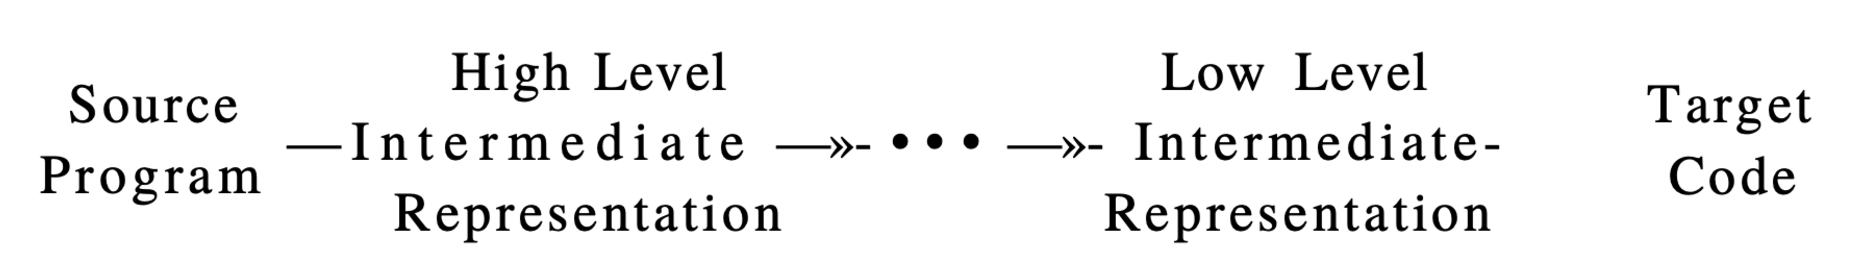
\includegraphics[width=.7\textwidth]{Imagens/abstraction-level-irs.eps}
  \caption{Sequência de representações intermediárias}\label{fig:abstraction-level-irs}
  \small{Fonte:~\cite{aho2008compilers}}
\end{figure}

Uma das principais informações que deve ser preservada em uma IR é o fluxo de controle, isto é, a ordem em que as instruções do programa são executadas, como chamadas de função, \textit{loops} e condições.
Para garantir que o compilador mantenha a semântica correta do programa, o fluxo de controle deve ser repassado de alguma maneira durante o processo de tradução~\cite{cooper2014construindo}.
Uma das maneiras disso ser feito explicitamente é com o uso de continuações, que são funções que descrevem o próximo passo de uma computação em um ponto particular da execução do programa.

\subsection{CPS}\label{subsec:cps}

O estilo de passagem de continuações (CPS, do inglês \textit{continuation passing style}) é uma técnica de transformação de código que torna o fluxo de controle de um programa explícito, ao converter o estilo convencional de chamadas de função em chamadas que passam explicitamente o controle para a próxima etapa, conhecida como continuação (do inglês, \textit{continuation})~\cite{appel1992compiling}.
Em vez de retornar diretamente o resultado de uma função, o CPS transforma cada função para que, ao finalizar sua computação, ela invoque uma continuação, que representa o próximo passo a ser executado no programa.
Assim, toda chamada de função se torna uma chamada de cauda.

Uma chamada de cauda (do inglês \textit{tail call}) ocorre quando a última instrução executada em uma função é uma chamada a outra função, sem que restem computações adicionais a serem feitas após essa chamada~\cite{muchnick1997advanced}.
Isso permite que a função atual libere seu quadro de ativação, otimizando o uso de memória, já que o compilador não precisa manter o estado da função anterior na pilha.
Em constraste, uma chamada que não é de cauda ocorre quando ainda restam operações após a chamada, como somas ou multiplicações, o que exige que o quadro de ativação da função atual permaneça na pilha até a conclusão dessas operações.

Na Figura~\ref{code:factorial_non_tail_call}, o exemplo da função fatorial demonstra uma chamada que não é de cauda, pois a chamada recursiva \texttt{factorial(n - 1)} não é a última operação a ser realizada.
A função precisa aguardar o retorno desta chamada para, então, multiplicar o resultado por \texttt{n}, o que impede a liberação do quadro de ativação até o término da multiplicação.

Em constrate, na Figura~\ref{code:factorial_tail_call} como exemplo, tem-se uma versão da função fatorial que utiliza chamada de cauda.
A função auxiliar \texttt{go} acumula o valor do cálculo diretamente em seu argumento \texttt{a}, e a chamada recursiva \texttt{go (n - 1) (a * n)} é a última instrução a ser executada.
Como não há operações pendentes após a chamada recursiva, o compilador pode otimizar a função, reutilizando o quadro de ativação da função \texttt{go} para a chamada subsequente, tornando o cálculo mais eficiente.

\lstinputlisting[style=haskell, label=code:factorial_non_tail_call, caption={Função fatorial em Haskell}]{Code/factorial_non_tail_call.hs}

\lstinputlisting[style=haskell, label=code:factorial_tail_call, caption={Função fatorial em Haskell com chamada de cauda}]{Code/factorial_tail_call.hs}

O cálculo lambda, definido por~\citeonline{church1932set}, é um sistema formal que serve como base para a maioria das linguagens funcionais.
Ele é capaz de representar qualquer computação utilizando abstrações e aplicações através de reduções.
Sua sintaxe consiste em três regras simples que definem os elementos principais do sistema: variável, abstração e aplicação, conforme apresentados a seguir:

\begin{equation}\label{eq:lambda-calculus}
  e ::= x \mid \lambda x. e \mid e e
\end{equation}

A partir dessa sintaxe, um termo $e$ pode possuir apenas uma das três formas.
A primeira forma refere-se às variáveis, que representam identificadores no sistema.
A segunda forma, chamada de abstração, define uma função lambda: uma função que associa o identificador $x$ a um termo $e$, seu corpo, com $x$ vinculado ao termo $e$.
Finalmente, a aplicação ocorre quando um termo $e$ é aplicado a outro $e$, representando a chamada de uma função.

No cálculo lambda, as variáveis podem ser classificadas como livres ou ligadas, dependendo de seu contexto em um termo.
Variáveis são consideradas livres quando não estão associadas a uma abstração de função.
Por exemplo, no termo $\lambda x. y$, a variável $y$ é livre, pois não está ligada a nenhum parâmetro introduzido.
Em contraste, no termo $(\lambda x. x) y$, a variável $x$ está ligada dentro do corpo da abstração, enquanto $y$ permanece livre.
Um termo sem variáveis livres é denominado fechado ou combinador; por exemplo, $\lambda x. \lambda y. x y$ é um combinador, pois todas as variáveis estão ligadas às suas respectivas abstrações.

Para avaliar expressões no cálculo lambda, usamos três tipos de redução: $\alpha$, $\beta$ e $\eta$, que seguem as seguintes definições:

\begin{description}
  \item[$\alpha$-redução:] Renomeação de variáveis ligadas.
        \begin{align}
          \lambda x . e & \rightarrow \lambda y . e[y/x]\label{eq:alpha-reduction}
        \end{align}
        Note que, $e[y/x]$ indica a substituição de todas as ocorrências ligadas de $x$ por $y$ em $e$, desde que $y$ não ocorra livre em $e$. Por exemplo, $\lambda x. x + z \rightarrow_\alpha \lambda y. y + z$.

  \item[$\beta$-redução:] Aplicação de função.
        \begin{align}
          (\lambda x . e_1) e_2 & \rightarrow e_1 [e_2 / x]\label{eq:beta-reduction}
        \end{align}
        Aqui, $e_1[e_2/x]$ denota a substituição de todas as ocorrências ligadas de $x$ em $e_1$ por $e_2$. Para evitar conflitos com variáveis livres em $e_2$, aplica-se $\alpha$-redução prévia. Por exemplo, em $(\lambda x. \lambda y. x + y)(y + 1)$, renomeia-se $y$ para $z$ na abstração interna:
        \[
          (\lambda x. \lambda z. x + z)(y + 1) \rightarrow_\beta \lambda z. (y + 1) + z.
        \]

  \item[$\eta$-redução:] Expansão de função.
        \begin{align}
          \lambda x . (e \, x) & \rightarrow_\eta e \quad \text{se } x \notin \text{FV}(e)\label{eq:eta-reduction}
        \end{align}
        Tal que $\text{FV}(e)$ denota as variáveis livres em $e$. Por exemplo, $\lambda x. (\lambda y. y + 1) \, x \rightarrow_\eta \lambda y. y + 1$.
\end{description}

As reduções são responsáveis pela semântica operacional do cálculo lambda.
A $\alpha$-redução permite a renomeação de variáveis ligadas, enquanto a $\beta$-redução descreve a aplicação de funções, substituindo o parâmetro da função por um valor passado como argumento.
Por fim, a $\eta$-redução lida com a simplificação de funções quando elas aplicam diretamente seu argumento.

A transformação para CPS se baseia nessa estrutura formal.
No cálculo lambda tradicional, o fluxo de execução é implícito: as funções são aplicadas e seus resultados são retornados automaticamente.
No entanto, no CPS, o fluxo de controle é explicitamente representado como uma série de chamadas a funções.
Cada função, em vez de retornar diretamente um valor, recebe um argumento extra, a continuação, que indica o próximo passo da computação.

Por exemplo, a expressão $\lambda x. x + 1$ no cálculo lambda tradicional retornaria o valor $x + 1$. Ao transformar essa expressão para CPS, ela se torna $\lambda x. \lambda k. k (x + 1)$.

Aqui, $k$ é a continuação que processa o resultado $x + 1$.
Ao converter funções para CPS, o fluxo de controle do programa passa a ser gerenciado de forma explícita através de chamadas de função que encadeiam as etapas subsequentes.
Essa transformação traz diversas vantagens no contexto de compiladores, pois torna explícitas as informações normalmente implícitas na pilha de execução e, assim, abre espaço para a aplicação de uma série de otimizações~\cite{appel1992compiling}.  

Em primeiro lugar, o CPS expõe todas as chamadas de cauda, permitindo a eliminação de recursividade em cauda (TCO, do inglês \textit{tail-call optimization}).
Essa otimização possibilita que chamadas recursivas sejam realizadas sem o acúmulo de quadros de ativação na pilha, reduzindo o uso de memória e evitando estouros de pilha em programas fortemente recursivos.

Além disso, a natureza explícita das chamadas em CPS favorece a expansão \textit{inline} de funções.
Como cada chamada é clara e separada, o compilador pode substituir uma chamada de função por sua definição diretamente, reduzindo o \textit{overhead} de chamadas e potencialmente expondo outras oportunidades de otimização.

Outro ponto importante é a representação de \textit{closures}.
Em CPS, como todo o contexto necessário à computação é passado de maneira explícita, o compilador consegue construir e manipular \textit{closures} com maior eficiência, uma vez que o ambiente da função está sempre disponível e bem definido.

A transformação para CPS também facilita a alocação de registradores.
Com o fluxo de controle explicitado, o compilador pode prever melhor o tempo de vida das variáveis e organizar os dados de forma que o uso de registradores seja maximizado e o número de acessos à memória minimizado~\cite{appel1992compiling}.

Por fim, como todo o fluxo de execução é expresso por chamadas encadeadas, o código gerado permite análises estáticas mais precisas.
O compilador pode, por exemplo, detectar com mais facilidade padrões de execução, dependências entre expressões e oportunidades de reordenação ou eliminação de código redundante.

Dessa forma, a conversão para CPS não apenas preserva a semântica da computação original, mas também fornece ao compilador uma estrutura rica e detalhada para aplicar otimizações de maneira eficaz.

O cálculo de continuações (do inglês, \textit{CPS-calculus}), conforme definido por~\citeonline{thielecke1997categorical}, é um sistema formal que leva o CPS além de seu uso tradicional como uma técnica de transformação de código, tratando-o como um modelo computacional por si só.
Enquanto o CPS é utilizado como uma IR em compiladores, o cálculo de continuações oferece uma estrutura para raciocinar formalmente sobre computações onde o fluxo de controle é explicitamente representado.
Os termos do cálculo de continuações, chamados de comandos, são descritos pelas seguintes regras:

\begin{equation}
  M ::= x\langle \vec{x} \rangle \mid M\{x\langle \vec{x} \rangle = M\}
\end{equation}

Aqui, $x\langle \vec{x} \rangle$ representa um salto (do inglês \textit{jump}), isto é, uma chamada para a continuação $x$ com os parâmetros $\vec{x}$, sendo essencialmente uma chamada direta para a continuação, enquanto $M\{x\langle \vec{x} \rangle = M\}$ representa um vínculo (do inglês \textit{binding}), onde o corpo $M$ está vinculado à continuação $x$ com os parâmetros $\vec{x}$, isto é, uma chamada intermediária que, ao ser chamada, executará o próximo passo da computação.
Vale ressaltar que \citeonline{appel1997shrinking} possuem uma sintaxe diferente para o cálculo de continuações, onde os termos são respectivamente representados como $k(\vec{x})$ e $\texttt{let }k(\vec{x}) = c \texttt{ in } b$.

A tradução para CPS converte um código escrito em estilo direto (onde o controle de fluxo é implícito) para o estilo de passagem de continuações~\cite{flanagan1993essence}.
A principal ideia por trás dessa transformação é modificar as funções para que elas não retornem um valor diretamente, mas, em vez disso, passem o resultado para uma continuação.

\lstinputlisting[style=haskell, label=code:add, caption={Função soma em Haskell em Estilo Direto}]{Code/add.hs}

\lstinputlisting[style=haskell, label=code:add_cps, caption={Função soma em Haskell em Estilo Direto}]{Code/add_cps.hs}

Por exemplo, a Figura~\ref{code:add} apresenta um programa na linguagem Haskell que soma dois números no estilo direto, retornando o valor após realizar o cálculo.
Já a Figura~\ref{code:add_cps} mostra um programa equivalente em CPS\@.
Nesta versão, o controle de fluxo do programa é explícito, pois a função $k$ é chamada para processar o resultado da soma dos argumentos.

\lstinputlisting[style=haskell, label=code:factorial, caption={Função fatorial em Haskell em Estilo Direto}]{Code/factorial.hs}

\lstinputlisting[style=haskell, label=code:factorial_cps, caption={Função fatorial em Haskell em CPS}]{Code/factorial_cps.hs}

Para ilustrar melhor, a Figura~\ref{code:factorial} apresenta um programa em Haskell que calcula o fatorial no estilo direto, utilizando funções definidas para multiplicação e subtração.
Na Figura~\ref{code:factorial_cps}, um programa similar em CPS é definido, com as funções auxiliares também transformadas para CPS\@.
Na função \texttt{factorialCps} é possível notar duas funções lambda (continuações), \texttt{nMinus1} e \texttt{factNMinus1}.
A primeira continuação guarda o resultado da operação $n - 1$, enquanto a segunda recebe recursivamente o cálculo do fatorial de $n - 1$, multiplica por $n$ e finalmente passa o resultado para a continuação $k$.

Outro fato importante a ser observado nos códigos apresentados é a tipagem das funções.
Na função de soma, definida na Figura~\ref{code:add}, a função tem tipo $Int \rightarrow Int \rightarrow Int$, ou seja, ela recebe dois inteiros e retorna um inteiro.
Já a função de soma em CPS, definida na Figura~\ref{code:add_cps}, possui o tipo $Int \rightarrow Int \rightarrow (Int \rightarrow r) \rightarrow r$. Isso significa que a função recebe dois inteiros e uma continuação, que é uma função de tipo $Int \rightarrow r$, onde \texttt{r} pode ser qualquer tipo, e retorna esse mesmo tipo \texttt{r}.

Essa transformação de tipo reflete a diferença fundamental entre o estilo direto e o CPS\@: em vez de retornar um valor diretamente, a função em CPS recebe uma continuação que especifica o próximo passo da computação.
O mesmo padrão pode ser observado nas funções para o cálculo do fatorial nas Figuras~\ref{code:factorial} e~\ref{code:factorial_cps}.
No estilo direto, a função \texttt{factorial} tem o tipo $Int \rightarrow Int$, enquanto na versão CPS, a função \texttt{factorialCps} tem o tipo $Int \rightarrow (Int \rightarrow r) \rightarrow r$.

Essa correspondência entre os tipos não é uma coincidência.
Como discutido por~\cite{torrens2019calculo}, uma função em estilo direto com tipo $A \rightarrow B$ pode ser transformada em uma função em CPS com o tipo $A \rightarrow (B \rightarrow \perp) \rightarrow \perp$.
Aqui, $\perp$ representa o tipo dos valores que nunca retornam, uma característica associada ao estilo de passagem de continuações, onde as funções são compostas de forma a encadear continuações até que a execução termine de maneira explícita.

Este exemplo simples da função fatorial em CPS ilustra as dificuldades inerentes ao uso de continuações explícitas, como a verbosidade do código, complexidade de compreensão e a propensão a erros.
No entanto, apesar desses desafios, o CPS se mostra extremamente adequado para a aplicação de otimizações, sendo uma escolha eficiente para representações intermediárias, especialmente em cenários onde o desempenho é essencial.

\section{Teoria de Tipos}\label{sec:type-theory}

A Teoria de Tipos, conforme apresentada por~\cite{COQUAND2022}, foi introduzida por Russell em 1908 ao encontrar um paradoxo na Teoria de Conjuntos, conhecido atualmente como o Paradoxo de Russell:

\begin{equation}\label{eq:russell-paradox}
  \text{Seja } R = \{ x \mid x \notin x \}, \text{ então } R \in R \iff R \notin R
\end{equation}

Ou seja, considere $R$ como o conjunto dos conjuntos que não contêm a si mesmos.
A contradição surge ao observar que, se o conjunto $R$ contém a si mesmo, isso implica que $R$ não contém a si mesmo, e vice-versa.

Outra maneira de descrever esse paradoxo é através do Paradoxo do Barbeiro: imagine uma cidade com apenas um barbeiro, onde ele somente barbeia aqueles que não se barbeiam.
O paradoxo surge quando perguntamos: ``Quem barbeia o barbeiro?''
Ele não pode fazer sua própria barba, pois barbeia apenas aqueles que não fazem a própria barba.
No entanto, se ele não faz sua própria barba, então pertence ao grupo daqueles que devem ser barbeados pelo barbeiro, logo, ele deveria barbear-se.
Essa situação gera uma contradição semelhante ao Paradoxo de Russell.

Atualmente, a principal aplicação da Teoria de Tipos está na formalização de sistemas de tipos para linguagens de programação.
Um sistema de tipos garante a ausência de certos comportamentos dos programas classificando os valores computados em cada uma de suas sentenças~\cite{PIERCE2002}.
Além disso, atribuir e verificar tipos para cada construção presente nos programas têm várias utilidades, como fornecer informações para auxiliar na modularização de programas, otimização de código executada pelo compilador e também pode ser usada como documentação do código.
Sistemas de tipos também são usados na construção de assistentes de provas, por exemplo, o Coq utiliza o Cálculo de Construções~\cite{COQUAND1998}.
Linguagens como Idris e Agda, que são funcionalmente dependentes, também permitem a verificação de provas formais.

No contexto das linguagens de programação, podemos distinguir três categorias principais de tipos: tipos simples, tipos polimórficos e tipos dependentes~\cite{PIERCE2002}.
Tipos simples atribuem um tipo fixo a cada termo, enquanto tipos polimórficos introduzem a noção de generalidade, permitindo que funções possam ser aplicadas a argumentos de diferentes tipos sem a necessidade de serem redefinidas para cada um.
Já os tipos dependentes permitem que tipos dependam de valores.

Um exemplo de tipo simples é uma função que opera sobre números inteiros.
Esta função recebe um número inteiro e retorna outro número inteiro.
Seu tipo, portanto, é representado como $Int \rightarrow Int$, indicando que tanto a entrada quanto a saída são do tipo inteiro.

Um exemplo de polimorfismo é a função identidade, que recebe um elemento de qualquer tipo e retorna o mesmo elemento.
Seu tipo é expresso como $a \rightarrow a$, onde $a$ pode ser qualquer tipo.
Este tipo polimórfico indica que a função identidade pode ser usada com diferentes tipos de dados sem precisar ser modificada.

Em linguagens com suporte a tipos dependentes, um exemplo seria o de um vetor cujo comprimento (número de elementos) faz parte de seu tipo.
Nesse caso, uma função de concatenação de vetores deve garantir que somente vetores com tipos compatíveis em relação ao comprimento possam ser concatenados.
O tipo da função de concatenação seria algo como\footnote{A notação exata pode variar entre diferentes linguagens de programação que suportam tipos dependentes. A estrutura apresentada serve apenas como uma ilustração conceitual do comportamento esperado.} $Vector(n) \rightarrow Vector(m) \rightarrow Vector(n+m)$, onde $n$ e $m$ são valores que representam os comprimentos dos vetores e fazem parte da definição de tipo.

No contexto do polimorfismo,~\citeonline{PIERCE2002} define duas principais variedades: o polimorfismo paramétrico, que permite que uma única definição de função opere de maneira genérica, e o polimorfismo com sobrecarga, que permite que uma função tenha diferentes comportamentos dependendo do tipo dos argumentos.
No polimorfismo paramétrico, como no caso da função identidade, todas as instâncias de uma função genérica compartilham o mesmo comportamento, independentemente dos tipos específicos com os quais são instanciadas.
Já no polimorfismo com sobrecarga, o comportamento da função pode variar conforme o tipo dos dados, como acontece com sobrecarga de operadores. Uma função sobrecarregada pode ter múltiplas implementações, com a seleção adequada dependendo dos tipos dos argumentos.

O polimorfismo desempenha um papel crucial na inferência de tipos.
Em linguagens com suporte a inferência de tipos, como Haskell, o sistema de tipos é capaz de deduzir tanto tipos específicos quanto tipos genéricos, sempre que possível, para permitir polimorfismo~\cite{PIERCE2002}.
O polimorfismo refere-se à capacidade de uma função ou expressão operar sobre diferentes tipos de dados de forma genérica.
Um exemplo clássico é a função identidade, $\lambda x.x$, que pode ser tipada como $\forall \alpha. \alpha \to \alpha$, indicando que a função aceita um valor de qualquer tipo $\alpha$ e retorna um valor do mesmo tipo.
Esse tipo é conhecido como polimorfismo universal~\cite{PIERCE2002}.

Já a função de soma apresentada na Figura~\ref{code:add} demonstra outro tipo de polimorfismo.
Como possui tipagem explícita $Int \rightarrow Int \rightarrow Int$, apenas valores do tipo inteiro podem ser somados.
No entanto, essa mesma função pode ser generalizada para permitir a soma de quaisquer números, desde que sejam do mesmo tipo, utilizando restrições de classe de tipos.

Em Haskell, uma classe de tipos é um conjunto de tipos que compartilham um conjunto comum de operações, e as classes de tipos são a maneira pela qual a linguagem lida com sobrecarga.
Por exemplo, a função \texttt{sumList}, que calcula a soma dos elementos de uma lista, pode ser definida com uma restrição de classe, na Figura~\ref{code:sum_list}.

\begin{figure}
  \caption{Função somatório de elementos de lista em Haskell}
  \small{Fonte: o autor}
  \lstinputlisting[style=haskell, label=code:sum_list]{Code/sum_list.hs}
\end{figure}

Aqui, a restrição \texttt{Num a} indica que \texttt{sumList} pode operar sobre listas de qualquer tipo \texttt{a}, desde que \texttt{a} pertença à classe \texttt{Num}, que define os tipos numéricos em Haskell.
Dessa forma, a função permite a soma de inteiros, valores \texttt{Float}, \texttt{Double} e outros tipos numéricos.

O polimorfismo restrito (ou polimorfismo de sobrecarga) é o que permite essa generalização~\cite{PIERCE2002}, pois a função é capaz de operar sobre múltiplos tipos, mas dentro de uma classe específica de tipos, garantindo flexibilidade e segurança no sistema de tipos.

O Cálculo Lambda Simplesmente Tipado é uma das primeiras e mais simples variantes do Cálculo Lambda que incorpora tipos em sua estrutura~\cite{CHURCH1940}.
Enquanto o cálculo lambda original não faz distinção entre diferentes tipos de dados, no Cálculo Lambda Simplesmente Tipado, os termos são anotados com tipos.
Cada função recebe e retorna valores de tipos específicos, o que permite prevenir uma série de erros comuns em programas, como a aplicação de funções a argumentos incorretos.

Além disso, o sistema de tipos serve como uma ferramenta de verificação durante a compilação de programas, assegurando que erros de tipo sejam detectados antes da execução.
Dessa forma, ele não apenas facilita a criação de software mais robusto, mas também oferece uma base formal para o estudo de linguagens de programação~\cite{PIERCE2002}.

A sintaxe básica do Cálculo Lambda Simplesmente Tipado inclui:

\begin{itemize}
  \item Variáveis: $x, y, z, \ldots$
  \item Tipos: $T ::= \mathbf{Int} \mid \mathbf{Bool} \mid T \to T$
  \item Termos: $\lambda x:T. \tau \mid \tau_1 \tau_2 \mid x$
\end{itemize}

No Cálculo Lambda Simplesmente Tipado, cada variável possui um tipo atribuído e os termos são construídos com base nesses tipos.
Por exemplo, a abstração de função $\lambda x:T. \tau$ define uma função onde a variável $x$ é de tipo $T$ e o corpo da função, $\tau$, é um termo.
A aplicação de função $\tau_1 \tau_2$ indica que $\tau_1$ é uma função que é aplicada ao argumento $\tau_2$, o qual deve ter um tipo compatível com o tipo esperado por $\tau_1$.

Essa formalização facilita a composição de funções e o raciocínio sobre a estrutura dos programas, pois cada termo pode ser avaliado dentro de um contexto de tipagem.
A sintaxe dos tipos, como $T \to T$, define uma função que aceita um argumento do tipo $T$ e retorna um valor também do tipo $T$.

A inferência de tipos no Cálculo Lambda Simplesmente Tipado assegura que cada expressão tenha um tipo bem-definido, baseado nas regras de tipagem.
A tipagem de termos é feita através de um conjunto de regras formais que garantem a consistência dos tipos no programa.
Por exemplo, a regra de tipagem para abstrações lambda é a seguinte:

\[
  \frac{\Gamma, x:T_1 \vdash \tau:T_2}{\Gamma \vdash (\lambda x:T_1. \tau): T_1 \to T_2}
\]

Isso significa que, se o termo $t$ possui o tipo $T_2$ sob o contexto onde $x$ possui o tipo $T_1$, então a abstração $\lambda x:T_1. \tau$ tem o tipo $T_1 \to T_2$.
Essa verificação de tipo garante que, ao aplicar a função, o tipo do argumento corresponde ao tipo esperado pela função.

O Cálculo Lambda Simplesmente Tipado está intimamente relacionado com a lógica intuicionista proposicional.
Esse vínculo é formalizado pela Correspondência Curry-Howard, que estabelece uma correspondência direta entre proposições lógicas e tipos, e entre provas e programas.
Em outras palavras, tipos podem ser interpretados como proposições lógicas, e termos tipados como provas dessas proposições~\cite{PIERCE2002}.

Por exemplo, o tipo $A \to B$ no Cálculo Lambda Simplesmente Tipado pode ser visto como a implicação lógica se $A$, então $B$.
Assim, uma função que aceita um argumento do tipo $A$ e retorna um valor do tipo $B$ é equivalente a uma prova de que $A$ implica em $B$.
Esse princípio permite usar ferramentas da teoria de tipos para construir provas formais de teoremas em lógica intuicionista, fornecendo uma base teórica robusta para assistentes de prova automatizados, como o Coq~\cite{COQUAND1998}.

Além disso, a Correspondência Curry-Howard não apenas conecta tipos e lógica, mas também oferece um método sistemático para projetar e raciocinar sobre sistemas de inferência de tipos, garantindo que programas tipados sejam corretos em relação às especificações lógicas.

A inferência de tipos desempenha um papel fundamental na programação funcional moderna, sendo inicialmente introduzida com a linguagem ML por~\citeonline{DAMAS1982}, com o algoritmo W.
A linguagem Haskell extende o sistema Damas-Milner, adicionando principalmente o suporte a sobrecarga de funções.

\section{Cálculo Lambda Simplesmente Tipado}\label{sec:simply-typed-lambda-calulus}

O Cálculo Lambda Simplesmente Tipado é uma das primeiras e mais simples variantes do Cálculo Lambda que incorpora tipos em sua estrutura~\cite{church1940formulation}.
Enquanto o cálculo lambda original não faz distinção entre diferentes tipos de dados, no Cálculo Lambda Simplesmente Tipado os termos são anotados com tipos.
Cada função recebe e retorna valores de tipos específicos, o que permite prevenir uma série de erros comuns em programas, como a aplicação de funções a argumentos incorretos.
Além disso, o sistema de tipos serve como uma ferramenta de verificação durante a compilação de programas, assegurando que erros de tipo sejam detectados antes da execução.
Dessa forma, ele não apenas facilita a criação de software mais robusto, mas também oferece uma base formal para o estudo de linguagens de programação~\cite{pierce2002types}.

A sintaxe básica do Cálculo Lambda Simplesmente Tipado inclui:

\begin{itemize}
  \item Variáveis: $x, y, z, \ldots$
  \item Tipos: $T \Coloneqq \mathbf{Int} \mid \mathbf{Bool} \mid T \to T$
  \item Termos: $\lambda x:T. \tau \mid \tau_1 \tau_2 \mid x$
\end{itemize}

No Cálculo Lambda Simplesmente Tipado, cada variável possui um tipo atribuído e os termos são construídos com base nesses tipos.
Por exemplo, a abstração de função $\lambda x:T. \tau$ define uma função onde a variável $x$ é de tipo $T$ e o corpo da função, $\tau$, é um termo.
A aplicação de função $\tau_1 \tau_2$ indica que $\tau_1$ é uma função que é aplicada ao argumento $\tau_2$, o qual deve ter um tipo compatível com o tipo esperado por $\tau_1$.
Essa formalização facilita a composição de funções e o raciocínio sobre a estrutura dos programas, pois cada termo pode ser avaliado dentro de um contexto de tipagem.
A sintaxe dos tipos, como $T \to T$, define uma função que aceita um argumento do tipo $T$ e retorna um valor também do tipo $T$.

A inferência de tipos no Cálculo Lambda Simplesmente Tipado assegura que cada expressão tenha um tipo bem-definido, baseado nas regras de tipagem.
A tipagem de termos é feita através de um conjunto de regras formais que garantem a consistência dos tipos no programa.
Por exemplo, a regra de tipagem para abstrações lambda é a seguinte:

\[
  \frac{\Gamma, x:T_1 \vdash \tau:T_2}{\Gamma \vdash (\lambda x:T_1. \tau): T_1 \to T_2}
\]

Isso significa que, se o termo $\tau$ possui o tipo $T_2$ sob o contexto onde $x$ possui o tipo $T_1$, então a abstração $\lambda x:T_1. \tau$ tem o tipo $T_1 \to T_2$.
Essa verificação de tipo garante que, ao aplicar a função, o tipo do argumento corresponde ao tipo esperado pela função.

O Cálculo Lambda Simplesmente Tipado está intimamente relacionado com a lógica intuicionista proposicional.
Esse vínculo é formalizado pela Correspondência Curry-Howard, que estabelece uma correspondência direta entre proposições lógicas e tipos, e entre provas e programas.
Em outras palavras, tipos podem ser interpretados como proposições lógicas, e termos tipados como provas dessas proposições~\cite{pierce2002types}.
Por exemplo, o tipo $A \to B$ no Cálculo Lambda Simplesmente Tipado pode ser visto como a implicação lógica ``se $A$, então $B$''.
Assim, uma função que aceita um argumento do tipo $A$ e retorna um valor do tipo $B$ é equivalente a uma prova de que $A$ implica em $B$.
Esse princípio permite usar ferramentas da teoria de tipos para construir provas formais de teoremas em lógica intuicionista, fornecendo uma base teórica robusta para assistentes de prova automatizados, como o Coq~\cite{coquand1988calculus}.

Além disso, a Correspondência Curry-Howard não apenas conecta tipos e lógica, mas também oferece um método sistemático para projetar e raciocinar sobre sistemas de inferência de tipos, garantindo que programas tipados sejam corretos em relação às especificações lógicas.
A inferência de tipos desempenha um papel fundamental na programação funcional moderna, sendo inicialmente introduzida com a linguagem ML por~\citeonline{damas1982principal}, com o algoritmo W.
A linguagem Haskell extende o sistema Damas-Milner, adicionando principalmente o suporte a sobrecarga de funções.

\newcommand{\defas}{\ensuremath{\overset{def}{=}}}
\newcommand{\fv}{\ensuremath{\text{FV}}}
\newcommand{\fvc}{\ensuremath{\text{FVC}}}
\newcommand{\eeq}{\ensuremath{\overset{e}{=}}}
\newcommand{\Append}{\ensuremath{\texttt{++}}}
\newcommand{\If}{\ensuremath{\text{se}}}
\newcommand{\Let}{\ensuremath{\text{let}}}
\newcommand{\In}{\ensuremath{\text{in}}}
\newcommand{\Then}{\ensuremath{\text{então}}}
\newcommand{\Return}{\ensuremath{\text{retorna}}}
\newcommand{\Else}{\ensuremath{\text{senão}}}
\newcommand{\Elseif}{\ensuremath{\text{senão se}}}
\newcommand{\Fail}{\ensuremath{\text{falha}}}
\newcommand{\Unify}{\ensuremath{\textit{unify}}}
\newcommand{\Occurs}{\ensuremath{\textit{occurs}}}
\newcommand{\True}{\ensuremath{\texttt{Verdadeiro}}}
\newcommand{\False}{\ensuremath{\texttt{Falso}}}
\newcommand{\Whitespace}{\ensuremath{\texttt{ }}}
\newcommand{\TODO}[1]{\textcolor{red}{\textbf{TODO:} #1}}

\section{Sistema Damas-Milner}\label{sec:damas-milner}

O sistema Damas-Milner, introduzido por Robin Milner e posteriormente formalizado em maior detalhe por Luis Damas~\cite{milner1978polymorphism,damas1982principal}, é um dos sistemas de tipos mais influentes para linguagens funcionais.
Este sistema tem como principal característica a inferência automática de tipos polimórficos, sem a necessidade de anotações explícitas por parte do programador, ocorrendo em linguagens como ML, Haskell e OCaml.
A sua base é o cálculo lambda com polimorfismo paramétrico, introduzido via \texttt{let}, permitindo que funções possam operar sobre múltiplos tipos de maneira genérica.

A introdução do sistema Damas-Milner trouxe duas contribuições principais: a definição de um sistema de tipos robusto e a criação de um algoritmo, o Algoritmo W, capaz de inferir o tipo mais geral (do inglês \textit{principal type-scheme}), conforme demonstrado em~\citeonline{damas1984assignment}.
O algoritmo é consistente e completo em relação ao sistema de tipos: a consistência assegura que todo tipo inferido é correto, ou seja, pode ser derivado pelo sistema de tipos; já a completude garante que qualquer tipo derivado pelo sistema será uma instância do tipo inferido pelo algoritmo.
Como resultado, a linguagem ML e suas derivadas se tornaram notórias por fornecer ao programador a capacidade de escrever programas sem erros de tipo detectáveis durante a compilação, permitindo um desenvolvimento mais seguro e robusto~\cite{milner1978polymorphism, damas1984assignment}.

A sintaxe do sistema Damas-Milner define as expressões e os tipos usados no processo de inferência.
Abaixo, segue a gramática das expressões e tipos:

\begin{equation}\label{eq:dm-syntax}\nonumber
  \begin{array}{ll}
    \text{Variáveis}         & x                                                                                 \\
    \text{Expressões}        & e \Coloneqq x \mid e \ e' \mid \lambda x.e \mid \texttt{let} \ x = e \ \texttt{in} \ e' \\
    \\
    \text{Variáveis de tipo} & \alpha                                                                            \\
    \text{Tipos primitivos}  & \iota                                                                             \\
    \text{Tipos}             & \tau \Coloneqq \alpha \mid \iota \mid \tau \rightarrow \tau'                       \\
    \text{Esquemas de tipo}           & \sigma \Coloneqq \forall \alpha. \sigma \mid \tau                        \\
  \end{array}
\end{equation}

Na sintaxe, $x$ representa variáveis que podem ser nomes de qualquer identificador, e $e$ descreve expressões que podem ser variáveis, aplicações de função, funções anônimas ou declarações \texttt{let}, que introduzem polimorfismo através de generalização de tipos.
$\alpha$ é usado para representar variáveis de tipos.
Os tipos primitivos $\iota$ são usados para representar tipos constantes.
Tipos $\tau$ podem ser tanto variáveis de tipo quanto funções entre tipos.
Por fim, $\sigma$ denota os esquemas de tipo (do inglês \textit{schemes}), ou tipos polimórficos, que podem quantificar variáveis de tipo, permitindo reutilização de variáveis de tipos em diferentes contextos.

O polimorfismo no sistema Damas-Milner é introduzido pelas expressões \texttt{let}, que permitem a generalização de tipos.
Ao declarar uma variável ou função usando \texttt{let}, o tipo inferido é generalizado para ser utilizado de maneira polimórfica na expressão que ocorre após o \texttt{in}.
Isso significa que, ao declarar uma função como $\texttt{let id} = \lambda x.x$, o sistema deduz o tipo mais geral $\forall \alpha. \alpha \rightarrow \alpha$, que pode ter sua variável de tipo $\alpha$ instanciada para diferentes tipos conforme for necessário.

A inferência de tipos envolve dois processos principais: generalização e instanciação.
A generalização ocorre quando o sistema identifica que uma expressão pode ser tipada com um tipo mais geral, permitindo que seja reutilizada de maneira polimórfica.
Já a instanciação ocorre quando um tipo polimórfico é aplicado a um tipo concreto, especializando-o para um uso específico.
Esse mecanismo garante a flexibilidade do sistema, ao mesmo tempo que mantém a segurança garantida pela inferência de tipos.
Por exemplo, considere a expressão $\texttt{let id} \ = \lambda x.x \ \texttt{in} \ (\texttt{id} \ \texttt{1}, \ \texttt{id} \ \texttt{`a'})$.
O sistema generaliza o tipo de $\texttt{id}$ para $\forall \alpha. \alpha \rightarrow \alpha$, e instancia este tipo tanto para inteiros quanto para caracteres nas duas aplicações subsequentes.

Outro conceito importante para o processo de inferência de tipos no sistema é a substituição de tipos, onde estes são mapeados para outros tipos ou para variáveis de tipo.
Formalmente, uma substituição de tipos é representada como um mapeamento finito de variáveis de tipo para tipos, denotado por $S$, e pode ser escrito na forma $[ \alpha_1 \mapsto \tau_1, \alpha_2 \mapsto \tau_2, \ldots, \alpha_n \mapsto \tau_n ]$.
Aqui, $\alpha_i$ são variáveis de tipo distintas e $\tau_i$ são os tipos correspondentes.
Em outras palavras, $S$ associa cada variável de tipo $\alpha_i$ a um tipo $\tau_i$ específico.

A aplicação de uma substituição $S$ em um tipo $\tau$, denotada por $S\tau$, resulta na substituição de todas as ocorrências livres de $\alpha_i$ em $\tau$ por $\tau_i$.
Esse conceito de substituição é fundamental para o processo de instanciação de tipos, que será discutido a seguir.
A definição formal da aplicação de substituições é dada por:

\begin{figure}[ht!]
  \centering
  \[
    \begin{array}{rcl}
      S\alpha_i                    & \equiv & \tau_i,                                                                          \\[8pt]
      S\alpha                      & \equiv & \alpha, \quad \text{se } \alpha \notin \{\alpha_1, \alpha_2, \ldots, \alpha_n\}, \\[8pt]
      S(\tau_1 \rightarrow \tau_2) & \equiv & S\tau_1 \rightarrow S\tau_2,                                                     \\[8pt]
      S(\forall \alpha.\sigma)     & \equiv & S' \sigma, \quad \text{onde } S' = S \setminus [\alpha \mapsto \_].
    \end{array}
    \]\label{fig:substituicao-tipos}
    \caption{Regras de aplicação da substituição de tipos}
    \small{Fonte:~\cite{castro2019certificacao}}
\end{figure}
\noindent onde o símbolo de subtração de conjuntos ($\setminus$) indica que a substituição $S'$ é a substituição $S$ restrita ao conjunto de mapeamentos que não envolvem a variável $\alpha$.

A instanciação de tipos é um processo em que um esquema de tipo $\sigma = \forall \alpha_1 \ldots \alpha_m. \tau$ é transformado em um tipo específico substituindo suas variáveis quantificadas por tipos concretos.
Se $S$ é uma substituição, então $S\sigma$ é o esquema de tipo obtido substituindo cada ocorrência livre de $\alpha_i$ em $\sigma$ por $\tau_i$, renomeando as variáveis genéricas de $\sigma$, se necessário.
O tipo resultante $S\sigma$ é chamado de uma instância de $\sigma$~\cite{damas1982principal}.
Esse processo é essencial para adaptar esquemas de tipos polimórficos a situações específicas em um programa, mantendo a flexibilidade e segurança do sistema de tipos.

Um esquema de tipo também pode ter uma instância genérica $\sigma' = \forall \beta_1 \ldots \beta_n. \tau'$, se existir uma substituição $[ \tau_i / \alpha_i ]$ tal que $\tau' = [\tau_i / \alpha_i]\tau$, e as variáveis $\beta_j$ não aparecem livres em $\sigma$.
Nesse caso, escrevemos $\sigma > \sigma'$, indicando que $\sigma$ é mais geral do que $\sigma'$.
Vale notar que a instanciação atua sobre variáveis livres, enquanto a instanciação genérica lida com variáveis ligadas.

O sistema de tipos de Damas e Milner é definido por um conjunto de regras de inferência de tipos, apresentadas na Figura~\ref{eq:type-inference}, que são usadas para determinar os tipos das expressões no sistema.
Essas regras são representadas por meio de julgamentos de tipos da forma $\Gamma \vdash e{:}\ \sigma$, onde $\Gamma$ é o contexto -- um conjunto de suposições na forma de pares $(x_i,\ \sigma_i)$, associando variáveis $x_i$ aos seus respectivos tipos $\sigma_i$ --, $e$ é a expressão sendo tipada, e $\sigma$ é o tipo inferido para essa expressão.

\begin{figure}[ht!]
  \fbox{$\Gamma\vdash x{:}\ \tau$}

  \centering

  \begin{prooftree}
      \LeftLabel{$\mathtt{[Taut]{:}\quad}$}
      \AxiomC{$x{:}\ \sigma \in \Gamma$}
      \UnaryInfC{$\Gamma \vdash x{:}\ \sigma$}
  \end{prooftree}

  \begin{prooftree}
      \LeftLabel{$\mathtt{[Abs]{:}\quad}$}
      \AxiomC{$\Gamma,\ x{:}\ \tau \vdash e{:}\ \tau'$}
      \UnaryInfC{$\Gamma \vdash (\lambda x.\ e){:}\ \tau \to \tau'$}
  \end{prooftree}

  \begin{prooftree}
      \LeftLabel{$\mathtt{[App]{:}\quad}$}
      \AxiomC{$\Gamma \vdash e{:}\ \tau' \to \tau$}
      \AxiomC{$\Gamma \vdash e'{:}\ \tau'$}
      \BinaryInfC{$\Gamma \vdash (e\ e'){:}\ \tau$}
  \end{prooftree}

  \begin{prooftree}
      \LeftLabel{$\mathtt{[Let]{:}\quad}$}
      \AxiomC{$\Gamma \vdash e{:}\ \sigma$}
      \AxiomC{$\Gamma, x{:}\ \sigma \vdash e'{:}\ \tau$}
      \BinaryInfC{$\Gamma \vdash (\texttt{let } x = e \ \texttt{in} \ e'){:}\ \tau$}
  \end{prooftree}

  \begin{prooftree}
      \LeftLabel{$\mathtt{[Inst]{:}\quad}$}
      \RightLabel{\scriptsize{$\mathtt{(\sigma\ \succ \sigma')}$}}
      \AxiomC{$\Gamma \vdash e{:}\ \sigma$}
      \UnaryInfC{$\Gamma \vdash e{:}\ \sigma'$}
  \end{prooftree}

  \begin{prooftree}
      \LeftLabel{$\mathtt{[Gen]{:}\quad}$}
      \RightLabel{\scriptsize $\alpha \notin \text{FV}(\Gamma)$}
      \AxiomC{$\Gamma \vdash e{:}\ \sigma$}
      \UnaryInfC{$\Gamma \vdash e{:}\ \forall \alpha.\ \sigma$}
  \end{prooftree}

  \caption{Regras de Inferência do sistema Damas-Milner}
  \small{Fonte: o autor. Adaptado de~\cite{damas1982principal}}\label{eq:type-inference}
\end{figure}

As regras de inferência são interpretadas de baixo para cima.
Por exemplo, na regra da tautologia \texttt{[Taut]} apresentada na Figura~\ref{eq:type-inference}, significa que, se em um contexto $\Gamma$, a variável $x$ possui o tipo $\sigma$, então podemos concluir que $x$ tem o tipo $\sigma$ no mesmo contexto.
Isso reflete o fato de que a associação de tipos no contexto é preservada.

Na regra de generalização \texttt{[Gen]} da Figura~\ref{eq:type-inference}, a condição de que $\alpha$ não seja livre em $\Gamma$ {---} formalmente escrita como $\alpha \notin \text{FV}(\Gamma)$ {---} assegura que o tipo generalizado não dependa de nenhum tipo específico presente no contexto.
Isso permite que o tipo $\forall \alpha.\ \sigma$ seja usado de forma polimórfica em diferentes partes do programa.

Essas regras garantem a solidez do sistema, preservando a segurança dos tipos ao inferir automaticamente os tipos mais gerais possíveis para as expressões.

Antes de apresentar o Algoritmo W, é importante observar que ele é uma implementação prática das regras de inferência aqui descritas, usando o conceito de unificação para resolver as equações de tipo geradas durante a inferência.
A seguir, será discutido em detalhes o funcionamento do Algoritmo W.

\subsection{Algoritmo W}\label{subsec:w-algo}

O Algoritmo W, introduzido em~\citeonline{damas1982principal}, é um algoritmo eficiente\footnote{Embora seja eficiente na grande maioria dos casos, há situações em que o Algoritmo W apresenta desempenho exponencial, conforme discutido em~\cite{vasconcellos2004inferencia}.} para inferência de tipos em linguagens de programação funcional.
Ele se baseia no processo de unificação para resolver equações de tipos geradas durante a análise de expressões, atribuindo a cada expressão um tipo principal (do inglês \textit{principal type-scheme}) (isto é, o tipo mais geral possível, no sentido de que qualquer outro tipo atribuível à expressão pode ser obtido a partir deste por substituição).
Formalmente, para uma expressão $e$, o Algoritmo W encontra um tipo $\tau$ tal que, para qualquer tipo $\tau'$ que também possa ser atribuído a $e$, existe uma substituição $S$ tal que $S(\tau) = \tau'$.

A unificação é o processo de encontrar uma substituição de variáveis de tipo que torna dois tipos dados equivalentes.
Formalmente, dados dois tipos $\tau_1$ e $\tau_2$, a unificação procura uma substituição $S$ tal que $S\tau_1 = S\tau_2$.
Se tal substituição existe, os tipos são considerados unificáveis e $S$ é chamada de solução unificadora.
Caso contrário, os tipos são incompatíveis.

O algoritmo de unificação, \Unify, descrito na Figura~\ref{algo:unify}, retorna a substituição que representa o unificador mais geral, operando recursivamente sobre a estrutura dos tipos.
Ele verifica se os tipos são idênticos, se uma variável de tipo pode ser substituída por outro tipo, ou, no caso de tipos compostos, se suas partes podem ser unificadas independentemente.

\begin{figure}[ht!]
  \centering
  \begin{align*}
     & \texttt{\Unify($\alpha, \Whitespace \alpha$) = }                                                                     \\
     & \qquad{}\texttt{\Return \Whitespace $[\Whitespace]$}                                                                 \\
     & \texttt{\Unify($\alpha, \Whitespace \tau)$ = }                                                                       \\
     & \qquad{}\texttt{\If \Whitespace \Occurs($\alpha, \Whitespace \tau$), \Then}                                          \\
     & \qquad{}\qquad{}\texttt{\Fail}                                                                                       \\
     & \qquad{}\texttt{\Else}                                                                                               \\
     & \qquad{}\qquad{}\texttt{\Return \Whitespace [$\alpha\mapsto\tau$]}                                                   \\
     & \texttt{\Unify($\tau, \Whitespace \alpha$) = }                                                                       \\
     & \qquad{}\texttt{\If \Whitespace \Occurs($\alpha, \Whitespace \tau$), \Then}                                          \\
     & \qquad{}\qquad{}\texttt{\Fail}                                                                                       \\
     & \qquad{}\texttt{\Else}                                                                                               \\
     & \qquad{}\qquad{}\texttt{\Return \Whitespace [$\alpha\mapsto\tau$]}                                                   \\
     & \texttt{\Unify($\tau_1 \to \tau_2, \Whitespace \tau_1' \to \tau_2'$) = }                                             \\
     & \qquad{}\texttt{\Return \Whitespace $\Unify(\tau_1, \Whitespace \tau_1') \circ \Unify(\tau_2, \Whitespace \tau_2')$}
  \end{align*}
  \caption{Algoritmo de unificação para o Sistema Damas-Milner no formato de função.}
  \small{Fonte: autor. Adaptado de~\cite{ribeiro2016mechanized}}\label{algo:unify}
\end{figure}

O algoritmo \Unify\ faz uso da função de verificação de ocorrência \Occurs\ apresentado na Figura~\ref{algo:occurs}, que por sua vez, tem como propósito evitar substituições que introduzam ciclos, como $[\alpha\mapsto\alpha\to\alpha]$, que resultaria em inconsistência no sistema de tipos~\cite{ribeiro2016mechanized}.
Esta função verifica recursivamente se uma variável de tipo $\alpha$ aparece em um tipo $\tau$.
Na última regra do algoritmo \Unify, ao unificar dois tipos função (do inglês \textit{arrow type}) $\tau_1 \to \tau_2$ e $\tau_1' \to \tau_2'$, a substituição resultante é obtida pela composição $S_2 \circ S_1$, onde $S_1 = \Unify(\tau_1,\ \tau_1')$ e $S_2 = \Unify(\tau_2,\ \tau_2')$.
Aqui, a composição $S_2 \circ S_1$ é definida como a substituição que aplica $S_1$ primeiro, seguida por $S_2$, ou seja, para qualquer variável de tipo $\alpha$, temos $(S_2 \circ S_1)(\alpha) = S_2(S_1(\alpha))$.
Essa definição garante que as substituições sejam aplicadas corretamente em cascata durante o processo de unificação.
\begin{figure}[ht!]
  \centering
  \begin{align*}
     & \texttt{\Occurs($\alpha, \Whitespace \tau_1 \to \tau_2$) = }                                                       \\
     & \qquad{}\texttt{\Return \Whitespace $\Occurs(\alpha, \Whitespace \tau_1) \lor \Occurs(\alpha, \Whitespace\tau_2)$} \\
     & \texttt{\Occurs($\alpha, \Whitespace \alpha$) = }                                                                  \\
     & \qquad{}\texttt{\Return \Whitespace \True}                                                                         \\
     & \texttt{\Occurs($\alpha, \Whitespace \tau$) = }                                                                    \\
     & \qquad{}\texttt{\Return \Whitespace \False}
  \end{align*}
  \caption{Algoritmo de verificação de ocorrência para o Sistema Damas-Milner no formato de função.}
  \small{Fonte: autor. Adaptado de~\cite{ribeiro2016mechanized}}\label{algo:occurs}
\end{figure}

O Algoritmo W, descrito na Figura~\ref{algo:w} é um método utilizado para inferência de tipos em expressões de linguagens funcionais.
Ele atribui os tipos mais gerais possíveis a cada subexpressão, garantindo a consistência com as operações definidas.
O algoritmo combina a unificação com regras de inferência de tipos para deduzir o tipo de uma expressão, explorando o polimorfismo de forma eficiente.

\begin{figure}[ht!]
  \fbox{$\Gamma \vdash_W e{:}\ \tau,\ S$}
  
  \begin{prooftree}
      \LeftLabel{\texttt{[Var]}}
      \AxiomC{$x{:}\ \sigma \in \Gamma$}
      \AxiomC{$\tau = \mathit{inst}(\sigma)$}
      \BinaryInfC{$\Gamma \vdash_W x{:}\ \tau,\ \emptyset$}
  \end{prooftree}

  \begin{prooftree}
      \LeftLabel{\texttt{[App]}}
      \AxiomC{$\Gamma \vdash_W e_0{:}\ \tau_0,\ S_0$}
      \AxiomC{$S_0\Gamma \vdash_W e_1{:}\ \tau_1,\ S_1$}
      \AxiomC{$\tau' = \mathit{newvar}$}
      \AxiomC{$S_2 = \mathtt{mgu}(S_1\tau_0,\ \tau_1 \rightarrow \tau')$}
      \QuaternaryInfC{$\Gamma \vdash_W e_0\ e_1{:}\ S_2\tau',\ S_2 S_1 S_0$}
  \end{prooftree}

  \begin{prooftree}
      \LeftLabel{\texttt{[Abs]}}
      \AxiomC{$\tau = \mathit{newvar}$}
      \AxiomC{$\Gamma,\ x{:}\ \tau \vdash_W e{:}\ \tau',\ S$}
      \BinaryInfC{$\Gamma \vdash_W \lambda x.\ e{:}\ S\tau \rightarrow \tau',\ S$}
  \end{prooftree}

  \begin{prooftree}
      \LeftLabel{\texttt{[Let]}}
      \AxiomC{$\Gamma \vdash_W e_0{:}\ \tau,\ S_0$}
      \AxiomC{$S_0\Gamma,\ x{:}\ \overline{S_0\Gamma}(\tau) \vdash_W e_1{:}\ \tau',\ S_1$}
      \BinaryInfC{$\Gamma \vdash_W \mathtt{let}\ x = e_0\ \mathtt{in}\ e_1{:}\ \tau',\ S_1 S_0$}
  \end{prooftree}

  \centering
  \caption{Algoritmo W em formato de regras de inferência.}
  \small{Fonte: o autor. Adaptado de~\cite{castro2019certificacao}}\label{algo:w}
\end{figure}

O funcionamento pode ser analisado para os diferentes tipos de expressões a seguir.
Para uma variável $x$ (regra \texttt{[Var]}), o algoritmo verifica se existe um esquema de tipo $\sigma$ associado a $x$ no contexto $\Gamma$.
Quando presente, realiza-se a instanciação de $\sigma$ substituindo suas variáveis quantificadas por tipos frescos (do inglês \textit{fresh types}) (variáveis novas sem colisões), obtendo o tipo concreto $\tau$.
A substituição identidade ($\emptyset$) é retornada com o tipo inferido.

Para aplicações de função $e_0\ e_1$ (regra \texttt{[App]}), o algoritmo primeiro infere recursivamente o tipo de $e_0$ em $\Gamma$, obtendo $\tau_0$ e a substituição $S_0$.
Em seguida, no contexto atualizado $S_0\Gamma$, infere o tipo de $e_1$ obtendo $\tau_1$ e $S_1$.
Um novo tipo variável fresco $\tau'$ é introduzido, e o unificador mais geral ($\mathtt{mgu}$) reconcilia $S_1\tau_0$ com $\tau_1 \rightarrow \tau'$, produzindo a substituição $S_2$.
O tipo resultante $S_2\tau'$ e a composição de substituições $S_2 \circ S_1 \circ S_0$ são retornados.

No caso de abstrações $\lambda x.e$ (regra \texttt{[Abs]}), um tipo fresco $\tau$ é gerado para $x$.
O contexto é estendido para $\Gamma,\ x{:}\ \tau$, e o tipo de $e$ é inferido nesse novo contexto, produzindo $\tau'$ e a substituição $S$.
O tipo da abstração é então determinado como $S\tau \rightarrow \tau'$, mantendo-se a substituição $S$.

Para expressões $\mathtt{let}\ x = e_0\ \mathtt{in}\ e_1$ (regra \texttt{[Let]}), o tipo de $e_0$ é inferido primeiro, resultando em $\tau$ e $S_0$.
O tipo $\tau$ é generalizado no contexto $S_0\Gamma$ através da operação $\overline{S_0\Gamma}(\tau)$, definida formalmente como:
\[
\overline{S_0\Gamma}(\tau) = \forall\ \hat{\alpha}.\ \tau \quad \text{onde} \quad \hat{\alpha} = \text{free}(\tau) - \text{free}(S_0\Gamma)
\]
ou seja, as variáveis de tipo $\hat{\alpha}$ (que são livres em $\tau$ mas não no contexto $S_0\Gamma$) são quantificadas, gerando um esquema de tipo polimórfico.
Este esquema é associado a $x$ ao inferir o tipo de $e_1$ no contexto $S_0\Gamma$, obtendo $\tau'$ e $S_1$.
O tipo final $\tau'$ e a composição $S_1 \circ S_0$ são retornados.


\chapter{Proposta}\label{ch:proposta}

\citeonline{thielecke1997} propôs um sistema de tipos monomórfico para CPS que define um único construtor (chamado de negação poliádica) para representar continuações \cite{TORRENS2024}:

% Imagens foda latex

\[
    \textit{Types } \ \tau \ ::= \ \neg \vec{\tau} \ \mid \ X
\]
\[
    \textit{Environments } \ \Gamma ::= \cdot \mid \Gamma, x : \tau
\]

\[
\frac{
  \Gamma(k) = \neg \vec{\tau} 
  \quad \quad
  \Gamma(\vec{x}) = \vec{\tau}
}{
  \Gamma \vdash k\langle \vec{x} \rangle
} \quad (J)
\]

\[
\frac{
  \Gamma, k : \neg \vec{\tau} \vdash b
  \quad \quad
  \Gamma, \vec{x} : \vec{\tau} \vdash c
}{
  \Gamma \vdash b \{ k \langle \vec{x} \rangle = c \}
} \quad (B)
\]

Enquanto uma sentença de tipos no sistema Damas-Milner: $\Gamma \vdash \text{e:}\tau$ declara que a expressão \texttt{e} possui tipo $\tau$ no contexto $\Gamma$, uma sentença de tipos: $\Gamma \vdash \text{b}$ declara que no contexto de tipos $\Gamma$, \texttt{b} é consistente.
Portanto $\{\text{x:}\tau \text{, k:} \neg \tau\} \vdash \text{k}\langle x \rangle$ estabelece que em um contexto em que \texttt{x} possui tipo $\tau$, \texttt{k} possui tipo $\neg \tau$, a expressão $\text{k}\langle \vec{x} \rangle$ não irá falhar~\cite{thielecke1997}.
\citeonline{TORRENS2024} demonstram a segurança (\textit{type safety}) desse sistema, provando preservação e progresso, ou seja, qualquer expressão bem tipada não apresentará comportamento inesperado quando reduzida.

O presente trabalho tem com objetivo propor uma extensão ao sistema proposto por Thielecke, adicionando o suporte a tipos polimórficos de forma similar ao que ocorre no sistema Damas-Milner.
Fornecendo também um algoritmo de inferência de tipos.
Por uma questão de tempo disponível, a validação do resultado será feita apenas de forma empírica por meio de testes.

Os próximos passos do trabalho proposto envolvem a formalização do sistema de tipos, bem como o desenvolvimento de um algoritmo de inferência para esse sistema.
Por fim, serão realizados testes com expressões de tipos conhecidos para validar a implementação.
A seguir, apresenta-se o cronograma previsto para a próxima fase deste trabalho.

\begin{enumerate}
	\item Formalização do sistema de tipos;\label{enum-formalizacao-sistema-tipos}
	\item Formalização do algoritmo de inferência;\label{enum-formalizacao-algoritmo}
	\item Implementação em Haskell, conforme definido nas Etapas~\ref{enum-formalizacao-sistema-tipos} e~\ref{enum-formalizacao-algoritmo};
	\item Validação dos resultados.
\end{enumerate}

\begin{table}[htbp]
	\centering
	\begin{tabular}{|c|c|c|c|c|c|c|c|c|}
		\hline
		\multirow{2}{*}{\textbf{\small{Etapas}}} & \textbf{\small{2024/1}} & \multicolumn{6}{c|}{\textbf{\small{2024/2}}} \\
		\cline{2-8}
		& \textbf{Dez} & \textbf{Jan} & \textbf{Fev} & \textbf{Mar} & \textbf{Abr} & \textbf{Maio} & \textbf{Jun} \\
		\hline
		\textbf{\small{1}}  & \cellcolor{gray} & \cellcolor{gray} & \cellcolor{gray} &  &  &  & \\
		\hline
		\textbf{\small{2}}  &  &  & \cellcolor{gray} & \cellcolor{gray} &  &  & \\
		\hline
		\textbf{\small{3}}  &  &  &  & \cellcolor{gray} & \cellcolor{gray} & \cellcolor{gray} & \\
		\hline
		\textbf{\small{4}}  &  &  &  &  &  & \cellcolor{gray} & \cellcolor{gray}\\
		\hline
	\end{tabular}
	\caption{Cronograma Proposto para o TCC2}
\end{table}
% \newcommand{\Mgu}{\ensuremath{\textit{mgu}}}
\newcommand{\MguList}{\ensuremath{\textit{mguList}}}
\newcommand{\UnifyVar}{\ensuremath{\textit{varBind}}}
\newcommand{\HeadSep}{\ensuremath{\textit{:}}}
\newcommand{\Length}{\ensuremath{\textit{length}}}
\newcommand{\List}{\ensuremath{\textit{list}}}


\section{Formalização}\label{sec:formalizacao}

Em razão da natureza mais prática deste trabalho, a notação utilizada para representar o cálculo de continuações será a mesma utilizada por~\citeonline{appel1997shrinking}, a sintaxe do `let'.
O sistema de tipos formalizado aqui foi fortemente inspirado no sistema de Damas e Milner, explicado na Seção~\ref{sec:damas-milner}, onde suas regras foram adaptadas de modo que elas se enquadrem no sistema polimórfico baseado em continuações.
Em particular, o contexto $\Gamma$ associa variáveis a tipos polimórfico e define julgamentos distintos para representar átomos e comandos.
A distinção destes se mostra necessária uma vez que é levado em consideração o comportamento não retornável das continuações. 

A sintaxe do sistema conta com expressões e tipos usados no processo de tipagem e de inferência de tipos.
Abaixo, segue a gramática das expressões e tipos presentes\footnote{Vale destacar que, todas as formalizações presentes aqui nesta seção, foram feitas pelo coorientador em reunião juntamente do autor, onde esse explicava suas motivações para atingir o resultado. Ainda, no momento da produção deste trabalho, não foi feita uma publicação contendo estas formalizações para que seja devidamente referenciada.}:

\phantom{Newline}

\begin{tabular}{lccl}
  Átomos & $a$ & $\Coloneqq$ & $x \enspace|\enspace n$ \\
  Comandos & $b$ & $\Coloneqq$ & $x(\vv{a}) \enspace|\enspace \mathtt{let}\ x(\vv{x}) = b\ \mathtt{in}\ b$ \\
  \\
  Tipos monomórficos & $\tau$ & $\Coloneqq$ & $\alpha \enspace|\enspace \mathtt{int} \enspace|\enspace \neg\vv{\tau}$ \\
  Tipos polimórficos & $\sigma$ & $\Coloneqq$ & $\forall\vv{\alpha}.\tau$ \\
  Contexto & $\Gamma$ & $\Coloneqq$ & $\cdot \enspace|\enspace \Gamma,\ x{:}\ \sigma$ \\
\end{tabular}\label{cps-type-system}

\phantom{Newline}

\noindent Na sintaxe apresentada, $a$ representa os átomos. Isto é, variáveis do programa ($x$) e literais inteiros ($n$) formam os elementos primitivos do sistema.
Os comandos $b$, por sua vez, são as expressões, explicadas com mais detalhes na Seção~\ref{subsec:cps}, sendo a primeira o \textit{jump}, e a segunda o \textit{bind}.
Três elementos distintos compõem os tipos presentes neste sistema.
Os tipos monomórficos ($\tau$), são os tipos que não possuem quantificação (monomórficos), podendo ser variáveis de tipo ($\alpha$), tipos numéricos inteiros ($\mathtt{int}$), ou ainda, tipos negados ($\neg\vv{\tau}$), usados para representar funções que retornam absurdos.
Já os tipos polimórfico ($\sigma$), são responsáveis por garantir a quantificação universal de variáveis de tipos (polimórficos).
Por fim, o contexto ($\Gamma$) contém o mapeamento de cada variável para um tipo polimórfico ($\sigma$).

As regras sintáticas de tipagem do sistema de tipos, inspiradas no Sistema Damas-Milner são ilustradas a seguir:

\phantom{Newline}

\fbox{$\Gamma\vdash a{:}\ \tau$}

\begin{prooftree}
    \RightLabel{$\mathtt{[Var]}$}
    \AxiomC{$x{:}\ \sigma \in \Gamma$}
    \AxiomC{$\sigma \sqsubseteq \tau$}
    \BinaryInfC{$\Gamma\vdash x{:}\ \tau$}
\end{prooftree}
\begin{prooftree}
    \RightLabel{$\mathtt{[Int]}$}
    \AxiomC{}
    \UnaryInfC{$\Gamma\vdash n{:}\ \mathtt{int}$}
\end{prooftree}

\phantom{Newline}

\fbox{$\Gamma\vdash b$}

\begin{prooftree}
    \RightLabel{$\mathtt{[Jump]}$}
    \AxiomC{$\Gamma\vdash k{:}\ \neg\vv\tau$}
    \AxiomC{$\Gamma\vdash \vv{a}{:}\ \vv{\tau}$}
    \BinaryInfC{$\Gamma\vdash k(\vv{a})$}
\end{prooftree}

\begin{prooftree}
    \RightLabel{$\mathtt{[Bind]}$}
    \AxiomC{$\Gamma, \vv{x}{:}\ \vv{\tau}\vdash c$}
    \AxiomC{$\Gamma,\ k{:}\ \overline{\Gamma}(\neg\vv\tau)\vdash b$}
    \BinaryInfC{$\Gamma\vdash\mathtt{let}\ k(\vv{x}) = c\ \mathtt{in}\ b$}
\end{prooftree}

Aqui, a regra $\mathtt{[Var]}$ define como tipo de uma variável uma instância do tipo (possivelmente polimórfico) que está associado a variável no contexto de tipos.
O símbolo $\sqsubseteq$ denota essa relação de ordem, indicando que o tipo $\tau$ é menos geral que $\sigma$.
Assim, em um contexto $\Gamma$, uma variável $x$ terá tipo $\tau$ caso esta esteja presente no contexto.
A regra $\mathtt{[Int]}$, é direta.
Em um contexto $\Gamma$, um literal inteiro terá um tipo $\mathtt{int}$.
Por exemplo, se $x{:}\ \forall\vv\alpha.\tau\in\Gamma$, então $\Gamma\vdash x{:}\ \tau$ (após instanciação adequada das variáveis de tipo).

As continuações, como discutido na Seção~\ref{subsec:cps}, representam fluxos de controle que não retornam valores.
Uma vez que a continuação pode ser interpretada como o próximo passo de uma computação, e a computação se dá por contradições, a continuação em si não possui um tipo, ela representa um absurdo.
Então, pode se dizer que a continuação é uma testemunha de que aquilo é um absurdo.

A regra $[\mathtt{Jump}]$ portanto, diz que sob um contexto $\Gamma$, se $k{:}\ \neg(\tau_1,\dots,\tau_n)$ com $n$ argumentos e cada argumento $a_i$ tiver um tipo correspondente $\tau_i$, então $k(\vv{a})$ é válido, ou seja, o salto $k$ com os argumentos $\vv{a}$ é testemunha de uma contradição.
De modo semelhante para o $\mathtt{[Bind]}$, as premissas $c$ e $b$ onde $c$ está sob o contexto $\{\ \Gamma\ \cup\ \{\ \vv{x}{:}\ \vv{\tau}\ \}\ \}$, e $b$ sob o contexto $\{\ \Gamma\ \cup\ \{\ k{:}\ \overline{\Gamma}(\neg\vv\tau)\ \}\ \}$, são testemunhas de que o comando $\mathtt{let}\ k(\vv{x}) = c\ \mathtt{in}\ b$ é uma contradição.
Assim como o `let' introduz o polimorfismo no sistema Damas-Milner, a generalização $\overline{\Gamma}(\neg\vv{\tau})$ presente na premissa do $\mathtt{[Bind]}$ quantifica as variáveis livres de $\vv{\tau}$ em $\Gamma$, estendendo o polimorfismo também ao CPS.

O algoritmo de inferência de tipos segue o mesmo esquema de Damas-Milner (algoritmo W) adaptado ao CPS.
Assim como o W, este faz uso do unificador mais geral, retornando sempre que existir o tipo mais genérico das expressões pertencentes a este sistema.
Abaixo, tem-se sua definição:

\phantom{Newline}

\fbox{$\Gamma\vdash_W a{:}\ \tau$}

\begin{prooftree}
    \AxiomC{$x{:}\ \sigma \in \Gamma$}
    \AxiomC{$\tau = \mathit{inst}(\sigma)$}
    \BinaryInfC{$\Gamma \vdash_W x{:}\ \tau$}
\end{prooftree}

\begin{prooftree}
    \AxiomC{}
    \UnaryInfC{$\Gamma \vdash_W n{:}\ \mathtt{int}$}
\end{prooftree}

\phantom{Newline}

\fbox{$\Gamma\vdash_W b \Rightarrow S$}

\begin{prooftree}
    \AxiomC{$\Gamma \vdash_W k{:}\ \tau_1$}
    \AxiomC{$\Gamma \vdash_W \vv{a}{:}\ \vv{\tau_2}$}
    \AxiomC{$S = \mathit{mgu}(\tau_1, \neg\vv{\tau_2})$}
    \TrinaryInfC{$\Gamma \vdash_W k(\vv{a}) \Rightarrow S$}
\end{prooftree}

\begin{prooftree}
    \AxiomC{$\vv{\tau} = \vv{\mathit{newvar}}$}
    \AxiomC{$\Gamma, \vv{x}{:}\ \vv{\tau} \vdash_W c \Rightarrow S_1$}
    \AxiomC{$\sigma = \overline{S_1\Gamma}(S_1 \neg\vv{\tau})$}
    \AxiomC{$S_1\Gamma, k{:}\ \sigma\vdash_W b \Rightarrow S_2$}
    \QuaternaryInfC{$\Gamma \vdash_W \mathtt{let}\ k(\vv{x}) = c\ \mathtt{in}\ b \Rightarrow S_2 \circ S_1$}
\end{prooftree}
Para as regras de inferência dos átomos, tal qual o sistema de tipos definido anteriormente, o algoritmo com uma variável $x$ de tipo polimórfico $\sigma$ pertencente ao contexto $\Gamma$ retornará um tipo monomórfico $\tau$ sob o mesmo contexto onde $\tau$ será a instanciação deste tipo $\sigma$.
Para o tipo numérico, não são necessárias premissas, algoritmo simplesmente devolve o tipo $\mathtt{int}$.
\begin{prooftree}
    \AxiomC{$a{:}\ \forall\alpha.\alpha \in \Gamma$}
    \AxiomC{$\alpha = \mathit{inst}(\forall\alpha.\alpha)$}
    \BinaryInfC{$\Gamma \vdash_W x{:}\ \alpha$}
\end{prooftree}
Por exemplo, esteja a variável $a$ com tipo $\forall\alpha.\alpha$ no contexto, ou seja, $a{:}\ \forall\alpha.\alpha\ \in\ \Gamma$.
O algoritmo então inferirá, que a variável $a$ terá tipo $\alpha$, após as devidas normalizações (redução-$\alpha$).

Os comandos serão inferidos a partir de substituições, onde o algoritmo as retornará representando o absurdo para qual esses testemunham.
Para o $\mathtt{[Jump]}$, partindo das premissas onde sob um contexto $\Gamma$, a chamada $k$ terá um tipo monomórfico $\tau_1$, os $n$ argumentos em $\vv{a}$ terão $n$ tipos monomórficos $\tau_2$, e ainda, $S$ é a unificação mais geral entre $\tau_1$ e $\neg\vv{\tau_2}$, o algoritmo irá então retornar esta substituição $S$ para o salto $k(\vv{a})$.

\begin{prooftree}
    \AxiomC{$\Gamma \vdash_W k{:}\ \alpha$}
    \AxiomC{$\Gamma \vdash_W x{:}\ \beta$}
    \AxiomC{$S = \mathit{mgu}(\alpha, \neg\beta)$}
    \TrinaryInfC{$\Gamma \vdash_W k(x) \Rightarrow \{\ \alpha \mapsto \neg\beta\ \}$}
\end{prooftree}
Por exemplo, em determinado contexto $\Gamma$, seja a chamada $k$ com tipo $\alpha$, ou seja, $\Gamma \vdash_W k{:}\ \alpha$, e ainda sob o mesmo contexto, o argumento $x$ com tipo $\beta$, ou seja, $\Gamma \vdash_W x{:}\ \beta$.
A partir da unificação mais geral entre $\alpha$ e $\neg\beta$ é obtida a substituição $S$, ou seja, $S = \mathit{mgu}(\alpha, \neg\beta)$.
O algoritmo então, irá inferir que a substituição para que o salto represente uma contradição é $\{\alpha \mapsto \neg\beta\}$.

Vale destacar que o algoritmo de unificação apresentado na Figura~\ref{algo:unify}, ainda que retorne a substituição que representa a unificação mais geral, não é o mesmo que o $\mathit{mgu}$ utilizado na regra $[\mathtt{Jump}]$.
Suas definições variam conforme os sistemas de tipos que elas atendem.
Enquanto que a função \Unify\ é definida para os tipos do Sistema Damas-Milner, a \Mgu, apresentada na Figura~\ref{algo:mgu-cps} é definida para os tipos do Sistema baseado em continuações.

\begin{figure}[ht!]
  \caption{Algoritmo de unificação para o Sistema baseado em continuações no formato de função.}
  \centering
  \begin{align*}
    & \texttt{\Mgu($\alpha,\Whitespace\tau$) = } \\
    & \qquad{} \texttt{\Return\Whitespace\UnifyVar($\alpha,\Whitespace\tau$)} \\
    & \texttt{\Mgu($\tau,\Whitespace\alpha$) = } \\
    & \qquad{} \texttt{\Return\Whitespace\UnifyVar($\alpha,\Whitespace\tau$)} \\
    & \texttt{\Mgu(\texttt{Int},\Whitespace\texttt{Int}) = } \\
    & \qquad{} \texttt{\Return\Whitespace[$\Whitespace$]} \\
    & \texttt{\Mgu(\texttt{Neg}\Whitespace ${list}_{1}$,\Whitespace\texttt{Neg} ${list}_{2}$) = } \\
    & \qquad{} \texttt{\If \Whitespace \Length\Whitespace${list}_{1}$ $\neq$ \Length\Whitespace${list}_{2}$, \Then \Whitespace \Fail} \\
    & \qquad{} \texttt{\Else\Whitespace\Return\Whitespace\MguList(${list}_{1},\Whitespace{list}_{2}$)} \\
    & \texttt{\Mgu($\tau_1,\Whitespace\tau_2$) = } \\
    & \qquad{} \texttt{\Fail} \\
    \\
    & \texttt{\MguList($[\Whitespace],\Whitespace[\Whitespace]$) = } \\
    & \qquad{} \texttt{\Return\Whitespace[$\Whitespace$]} \\
    & \texttt{\MguList($[\tau\HeadSep\Whitespace\tau_s],\Whitespace[\tau'\HeadSep\Whitespace\tau_s']$) = } \\
    & \qquad{} \texttt{$S_1$\Whitespace:=\Whitespace\Mgu($\tau,\Whitespace\tau'$)} \\
    & \qquad{} \texttt{$S_2$\Whitespace:=\Whitespace\MguList($S_1(\tau_s),\Whitespace S_1(\tau_s')$)} \\
    & \qquad{} \texttt{\Return\Whitespace$S_2\Whitespace \circ\Whitespace S_1$} \\
    & \texttt{\MguList($\_,\Whitespace\_$) = } \\
    & \qquad{} \texttt{\Fail}
  \end{align*}
  \small{Fonte: autor.}
  \label{algo:mgu-cps}
\end{figure}

A principal diferença deste algoritmo em relação ao anterior é que, neste sistema de tipos, há listas de tipos que também precisam ser unificadas.
Para realizar essa unificação, verifica-se inicialmente se as duas listas possuem o mesmo tamanho, ou seja, se $\texttt{\Length}\ list_1 = \texttt{\Length}\ list_2$.
Caso essa condição seja satisfeita, o algoritmo \Mgu\ é aplicado recursivamente a cada par de tipos correspondentes nos mesmos índices das listas, acumulando as substituições parciais ao longo do processo.
A função \texttt{\UnifyVar} é responsável por realizar a unificação entre variáveis de tipo e outros tipos, retornando a substituição correspondente ou um erro, caso a verificação de ocorrência via \texttt{\Occurs} falhe.

Para a regra que garante o polimorfismo do sistema, o $[\mathtt{Bind}]$, a chamada $k$ recebe $\vv{x}$ argumentos, onde estes terão $\vv{\tau}$ tipos como sendo variáveis de tipo, ou seja, $\vv{\tau} = \vv{\mathit{newvar}}$.
O $c$, por se tratar de um comando, será uma substituição $S_1$, onde recursivamente será inferida com o contexto inicial $\Gamma$ unido com os $\vv{x}$ argumentos tipados com suas $\vv{\tau}$ variáveis de tipo frescas, ou seja, $\{\ \Gamma\ \cup\ \{\ \vv{x}{:}\ \vv{\tau}\ \}\ \} \vdash_W c \Rightarrow S_1$.
Um ponto de atenção é necessário na função de generalização $\sigma = \overline{S_1\Gamma}(S_1 \neg\vv{\tau})$.
A subsituição $S_1$ aplicada no contexto garante que este esteja atualizado com a descoberta do comando $c$ na premissa anterior.
Como as continuações não retornam e sim somente passam o resultado da computação adiante, é necessário também que $S_1$ seja aplicado no tipo do argumento $S_1 \neg\vv{\tau}$, para garantir que a substituição obtida no comando anterior seja utilizada nos tipos.
De maneira semelhante ao primeiro comando, o comando $b$ é inferido recursivamente com $S_1$ aplicado no contexto unido com o salto $k$ tendo o tipo polimórfico $\sigma$ produzido na premissa anterior, sendo atribuido a esta inferência a substituição $S_2$, ou seja, $\{\ S_1\Gamma\ \cup\ \{\ k{:}\ \sigma \ \} \ \} \Rightarrow S_2$.
O algoritmo portanto, para o comando $\mathtt{let}\ k(\vv{x}) = c\ \mathtt{in}\ b$, irá produzir a substituição resultante da composição entre as substituições de $b$ e $c$, ou seja, $S_2 \circ S_2$.

% \section{Implementação}\label{sec:implementacao}
% \begin{frame}{Conclusões Parciais}
    \begin{itemize}
        \item CPS é uma escolha interessante para IR
              \begin{itemize}
                  \item Otimizações
              \end{itemize}
        \item Sistema de tipos
              \begin{itemize}
                  \item Correção de transformações e otimizações
                  \item Ausência de certos comportamentos indesejados
              \end{itemize}
    \end{itemize}
\end{frame}



\postextual%

% Referências bibliográficas
\bibliography{bibliography}										% Elemento Obrigatório

%\include{PosTextuais/Glossario}							% Elemento Opcional
%\include{PosTextuais/Apendices}							% Elemento Opcional
%\include{PosTextuais/Anexos}									% Elemento Opcional
%\include{PosTextuais/IndiceRemissivo}				% Elemento Opcional

\end{document}
